\documentclass[prodmode]{acmlarge}

\raggedbottom

\usepackage[numbers, square,sort&compress]{natbib}
\bibliographystyle{abbrvnat}
\renewcommand{\bibnumfmt}[1]{#1}
%\bibpunct{}{}{}{n}{}{}

% Metadata Information
% Not used, but required by template.
\acmVolume{2}
\acmNumber{3}
\acmArticle{2}
\articleSeq{2}
\acmYear{2010}
\acmMonth{5}
\usepackage{color}
%\usepackage{listings}

\usepackage{url}
\usepackage{fancyvrb}
\usepackage{listings}
\usepackage{caption}


\usepackage[T1]{fontenc}
\usepackage{inconsolata}

\definecolor{offwhite}{gray}{0.96}


\makeatletter
%% define a caption format; if the caption
%% is the default (\relax), the separator is
%% not printed; as long as no caption text
%% starts with \relax, this will work
\DeclareCaptionFormat{alsoempty}{%
  #1\if\relax\expandafter\noexpand\lst@caption\else#2#3\fi}

\DeclareCaptionFormat{figalsoempty}{%
  #1\if\relax\expandafter\noexpand\@caption\else#2#3\fi}
\makeatother

\lstset{
  fancyvrb=true,
  basicstyle=\ttfamily\footnotesize,
  captionpos=b,
  xleftmargin=2em,
  caption=\relax,
  backgroundcolor=\color{offwhite},
  mathescape}

\lstnewenvironment{snippet}[1][]{
    \renewcommand*{\lstlistingname}{Snippet}
    \minipage{\linewidth}
    \lstset{#1}
}{\endminipage}

\captionsetup[lstlisting]{format=alsoempty,font=footnotesize}
%\captionsetup[figure]{format=figalsoempty}

%\renewcommand{\artnum}{}
%\renewcommand{\firstfoot}{}

% Title portion
\title{Sigma: Android Binder Services over Network}
\author{KASTURI RANGAN RAGHAVAN~~~
Supervisor: MANI SRIVASTAVA\\
MS Comprehensive Project~~~
University of California, Los Angeles
}
%\terms{}

\begin{document}
\pagestyle{plain}
\maketitle
\tableofcontents

\clearpage

\section{Abstract}
The Android mobile platform is built on a service-oriented architecture. Yet there are no idiomatic mechanisms to provide local services to remote Android clients. Current Android services are provided with an underlying message-based interprocess-communication (IPC) protocol--known as Binder--implemented as a linux kernel module. Binder messages transit through the kernel module and often contain local descriptors--pointers to kernel-managed Binder objects or file descriptors.

This paper introduces Sigma, an experimental protocol supporting the tunneling of Binder messages over network connections. Sigma inspects and rewrites Binder messages containing descriptors, providing operations on those descriptors over the network. Thus, Android services relying on Binder are supported over the network, even enabling access to system services.

We implement Sigma over HTTP- and XMPP-based network connections, evaluating the ability to access services such as sensor and location updates between Android devices. Treating every Sigma-enabled device as a peer in a network, Sigma transforms the Android mobile platform into a platform for distributed applications. To demonstrate, we design a simple picture sharing service purely with Binder and show how, with the help of Sigma, it can become a distributed application.

\section{Introduction and Problem Definition}

The Android mobile platform is built on a service-oriented architecture. Yet there are no idiomatic mechanisms to provide local services to remote Android clients. This paper introduces Sigma, an experimental platform that builds upon Android's service-oriented runtime to allow tunneling of Android services over network connections. Sigma makes communication between devices a responsibility of the mobile platform. All binder services are supported over the network, even enabling access to system services. Treating every Sigma-enabled device as a peer in a network, Sigma transforms the Android mobile platform into a platform for distributed applications.

\subsection{Mobile Apps as Distributed Apps}
As motivation, we now discuss a relevant set of mobile applications which can be implemented via the distributed communication model rather than the traditional client-server model.

\subsubsection{Social Apps}
A niche of social services, especially those that connect small sets of participants together for brief periods of time are good candidates for the distributed communication model. These services require a central server only occasionally--for tasks such as to authenticate or to establish an initial network among participants. Voice and video chat applications are good examples. Even today, these apps typically use a direct peer-to-peer (P2P) connection among participants once a chat session is established~\cite{SkypeStudy,GoogleTalkLibrary}.

The use of real-time context has gained popularity among social apps. There are a whole crop of location sharing apps that give users a glimpse into a small set of friends' location and activities. Apps like Find My Friends~\cite{FindMyFriends} for iOS or Glympse~\cite{Glympse} for Android. Although it is not known whether these closed-source apps use a peer-to-peer or client-server approach (probably the latter), from their functionality alone it seems feasible to implement with the former model. The basic usefulness is garnered from the streaming of real-time data from participants' mobile devices, and therefore a prerequisite is that all active participants must be reachable over the network. It follows that participants must be able to establish P2P connections too. Also, such services do not need access to historical data, so we can do without a central server's storage and serving capacity.

An emerging class of social apps is characterized by the sharing of ephemeral data. The most popular service being Snapchat--a photo messaging app where recipients see the photos shared with them for a brief period (1 to 10 seconds) and then it disappears~\cite{Snapchat}. The nature of the service is one that affords participants some privacy.

``Snapchat is a super interesting privacy phenomenon because it creates a new kind of space to communicate, which makes it so that things that people previously would not have been able to share, you now feel like you have place to do so,'' says Mark Zuckerberg--CEO of Facebook. ``That's really important, and that's a big kind of innovation that we're going to keep pushing on and keep trying to do more on, and I think a lot of other companies will, too.''~\cite{Zuckerberg}

However, Snapchat follows a client-server model today. This much is known, because a security breach~\cite{SnapchatHack} at Snapchat established that shared pictures (thought to be privately shared and ephemeral) are stored by Snapchat servers long after they have been viewed by recipients. A truly privacy-aware implementation of Snapchat would use a pure P2P approach. If distributed communication is well-supported by the mobile platform, it encourages developers create applications following that model. A simple implementation of a picture sharing service implemented as a distributed application (with the help of Sigma to provide communication between devices) is demonstrated in section~\ref{sec:ExampleApplication}

\subsubsection{Internet of Things}
Distributed communication is a valuable model in the Internet of Things (IoT). It is likely that Android will be a major player in the IoT. Already consumer products like the \$30 Chromecast--a bare-bones Android device that plugs into the HDMI port of TVs--is capable of receiving video and display streams from other Android devices over LAN~\cite{chromecast}. Chromecast communicates with other Android devices using webrtc, an emerging W3C P2P standard~\cite{ChromecastWebrtc}. Future internet-enabled home appliances will probably use Android in some form~\cite{AndroidEverywhere}. And the idea of a ``smart home'' is taking off. Google, being the main driver of Android today, recently acquired Nest~\cite{GoogleNest}--a company that formerly developed smart home thermostats.

The IoT is filled with problems of communication between devices. For example, in the smart home an Android-enabled thermostat might poll for sensor readings like temperature and humidity from a mobile Android device in the home. We see already a crop of frameworks--like the Eclipse M2M stack for distributed communication between embedded devices~\cite{eclipse_m2m} that primarily uses the the publish-subscribe pattern~\cite{PublishSubscribe}. Although publish-subscribe is a simple, easy-to-understand model, the Android service-oriented architecture is more than that (as we will see in later sections). Therefore it is interesting to experiment with the Android service-oriented architecture as a model for distributed communication, especially when concerning ourselves with communication exclusively between Android-enabled devices in the IoT.

\subsection{Related work}
There are standard implementations of P2P technologies and networking libraries. Naturally, these implementations exist outside of the Android Runtime. Sigma aims to use these standard technologies, but to create a distributed communication model that is a better fit within Android. There is prior work in Academia very similar to this paper. To give just one example: the Interdroid~\cite{Interdroid} project also aims to create a platform for distributed applications on Android. However Interdroid defines a separate API for distributed communication that apps must conform to, much like the Eclipse M2M specifies its own publish-subscribe API. Related more to the creation of privacy-aware apps is $\pi$Box~\cite{piBox}: a platform for privacy-preserving apps, achieving a sandbox that spans across devices, providing secure channels. Since $\pi$Box targets Android, it fits the Android model better than standard third-party libraries. However, distributed communication requires the reimplementation of apps using the concept of the secure channels. In comparison, Sigma is an attempt at generalizing the existing Android service-oriented architecture. In creating distributed apps, the existing programmer support provided in the Android SDK for creating local service-oriented apps can be leveraged. No previous project, to the best of our knowledge, enables distributed communication on Android using Android's very own service-oriented runtime.

The inspiration for this paper is in part from the well-known X windows system. X is a server that manages display and input-device operations. Applications connect to X and follow a simple protocol (X11) to create and coordinate GUI interactions. It is a fully message-based protocol, and is specifically designed to allow for messages to be tunneled through network connections~\cite{X11}. This allows applications running on one machine to be displayed and controlled via a remote X server. Thus, anyone with an interactive terminal (e.g. ssh) to a machine can interact with GUI applications via X11-forwarding. Sigma aims to accomplish something similar for Android Services.

\subsection{Problem definition}

The goal of Sigma is to provide Android services over network connections. Current Android services are provided with an underlying message-based interprocess-communication (IPC) protocol known as Binder. It is implemented as a linux kernel module. Binder is message-based, but messages transit through the kernel module and often contain local descriptors--pointers to other binder services or file descriptors managed by the kernel module. As such, Binder is not designed to be tunneled over network connections, and there is no such existing facility for it. Sigma is introduced as a protocol and then an implementation. It is designed as a message-based protocol that aims to support a subset of Binder. Its design and implementation is specifically made to support tunneling over network connections. Sigma inspects and rewrites Binder messages containing descriptors, providing operations on descriptors over the network.

This paper explores the Binder framework in depth, and then provides the design and implementation of Sigma. The rest of the paper is organized as follows. Section~\ref{sec:AndroidBinderFramework} is an overview of Binder from its kernel module implementation to its object-oriented (OO) implementation in the Android Runtime. Next, Section~\ref{sec:SystemServices} is an overview of the implementation of a few Android system services, with a discussion on which services make sense to provide over the network. Then the design and implementation detail of Sigma is presented in Section~\ref{sec:Sigma}, presenting an overall design idea followed by a systematic implementation detail of each piece. We evaluate overhead and test performance in Section~\ref{sec:Performance}: first with some simple binder services and then with Android system services. As an example of a distributed application built from the ground-up, in Section~\ref{sec:ExampleApplication} we develop a simple picture sharing service using purely Binder services--made into distributed app with the help of Sigma. Finally, Section~\ref{sec:Discussion} contains discussion and next steps, particularly detailing limitations and drawbacks and what we can do to fix them.

\section{The Android Binder Framework}
\label{sec:AndroidBinderFramework}
The Binder framework is Android's primary IPC mechanism, and it is used widely within the Android Runtime. System services are provided through binder. A binder allows a process to present a specific interface as a service which may be called by other threads or processes. A binder call is essentially a remote procedure call (RPC) with communication between linux processes achieved using ioctl calls on a file descriptor. The binder at its most basic level is a kernel module. As such binder maintains isolation between processes, maintaining modularity and privilege separation as implemented by the linux kernel~\cite{OpenBinder}.

\subsection{Kernel Module}
The binder kernel module (BKM) provides the facility to register a default binder service known as the context manager. It is then the job of the context manager to manage binder objects in the operating system. This context manager can be accessed by arbitrary processes via a call to the BKM. In Android the context manager presents an IServiceManager interface which provides actions to manage a directory of system services, and where system services publish themselves to the directory via binder RPC.

Using the lowest-level C API for communicating with the BKM, here are the sequence of commands to create and publish a binder service. The binder service is implemented via a handler function, and incoming requests invoke it. The body of the handler function is not shown here. The arguments to binder\_call are described in the Appendix~\ref{app:binder_call}. This binder\_call is targeted at the ServiceManager, and invokes its handler function running on the root system process.

\begin{snippet}[label=snip:binder_call,caption=binder\_call to publish a service with ServiceManager]
binder_state* binder_service = binder_open();
binder_state* publish_txn = binder_open();

// RPC to the ServiceManager to publish the  service, details of
// arguments to binder_call  are described in the appendix.
binder_call(publish_txn, msg, reply, (void*)0, SVC_MGR_ADD_SERVICE);

// loop indefinitely. Incoming transactions  will invoke the handler.
binder_loop(binder_service, (void*)service_handler);
\end{snippet}

Note that msg and reply are binder\_io data structures (see Appendix~\ref{app:binder_io}) that contain the data to be passed into or returned, respectively, from binder\_call. All actions on a binder service are implemented through binder\_call, and the contents of binder\_io to complete a particular action is matter of convention. In the above example to publish a service to ServiceManager, the binder\_io msg contains the following elements, with the data encoded into a flat byte array. The 2 strings and 1 object are read in the same order by handler function of ServiceManager.

\begin{snippet}[caption=contents of msg passed into binder\_call]
msg = {
  "android.os.IServiceManager" /* string name of the remote interface */,
  "com.example.service" /* string name of service being published */,
  object /* flat_binder_object struct with pointer to binder_service */
}
\end{snippet}

Another process can obtain a handle to the just-published service via a binder RPC to ServiceManager, this time supplying a different code (SVC\_MGR\_GET\_SERVICE) denoting a different remote action, and msg containing the name of service to retrieve. The return value (the reply) will contain a descriptor--the handle to the remote binder service.

Invoking a binder RPC targeted at this new handle will invoke the associated service handler. The interaction between the kernel module and other processes is visualized below in figure~\ref{fig:binder_call}.

\begin{figure}[h]
\centering
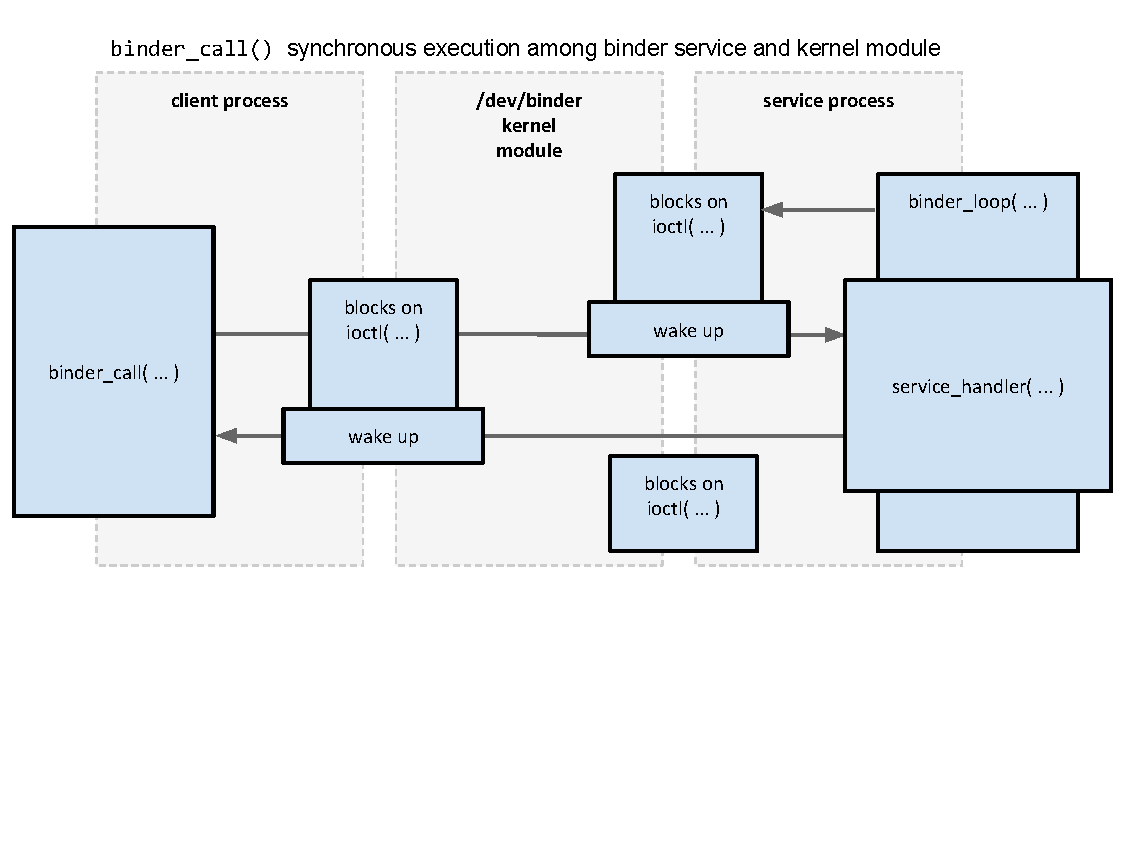
\includegraphics[width=\textwidth]{drawings/binder_call.pdf}
\caption{binder\_call synchronous IPC execution among binder service and kernel module}
\label{fig:binder_call}
\end{figure}

\subsubsection{binder\_io with objects and file descriptors}
An essential feature of binder is the ability to write binder objects and file descriptors as arguments into (or in replies from) RPCs. A handle to an binder object is a descriptor that is tracked by the kernel module, and the binder driver takes care of rewriting the structure type and data as it moves between processes~\cite{BinderSourceComment}. A process can obtain a handle to a remote binder service, and can invoke a RPC on the object. As evident from the above communication with ServiceManager, this feature is used to publish and then retrieve binder services among processes. Both primitive types and objects are written into the binder\_io structure, encoded as a byte-array.

This level of understanding of BKM is sufficient in detail for the scope of this paper. Documentation on internals of binder is sparse. The following references~\cite{BinderLinuxFoundation,BinderMastersThesis} provide a useful resource, but the real reference to Binder is in code--its implementation in Android.

\subsection{Binder within the Android Runtime}
The Android Runtime has several layers of abstractions built on top of the BKM. All these layers eventually result in calls either to the lowest-level C API which we have just covered or directly operate on the kernel driver. The main difference is that the C++ and Java APIs are object-oriented (OO), defining an IBinder interface which binder services implement. transact(...) is the method to perform generic operations to implement RPC. It very much resembles the low-level C API's binder\_call(...) function. The OO implementation also encapsulates binder\_io structures as Parcel objects.

\begin{snippet}[label=snip:IBinder]
interface IBinder {
  // Get the canonical name of the interface supported by this binder.
  String getInterfaceDescriptor();
  boolean transact(int code, Parcel data, Parcel reply, int flags);
  void linkToDeath(DeathRecipient recipient, int flags);
  boolean unlinkToDeath(DeathRecipient recipient, int flags);
  // ... among other methods
}
\end{snippet}

The OO Binder follows the Proxy Pattern~\cite{ProxyPattern}. BBinder is a class that is instantiated as the real implementation of the service. It invokes and waits on the equivalent of binder\_loop and accepts transaction requests. Then there is BpBinder which is a proxy class that is instantiated with a remote handle to an active BBinder service. Analogously, there is a Java implementation that has a mirror IBinder interface, and defines Binder and BinderProxy Java classes which encapsulate the native BBinder and BpBinder classes, respectively, via JNI. The Java IBinder interface is provided in Snippet~\ref{snip:IBinder}.

%\begin{figure*}
%\centering
%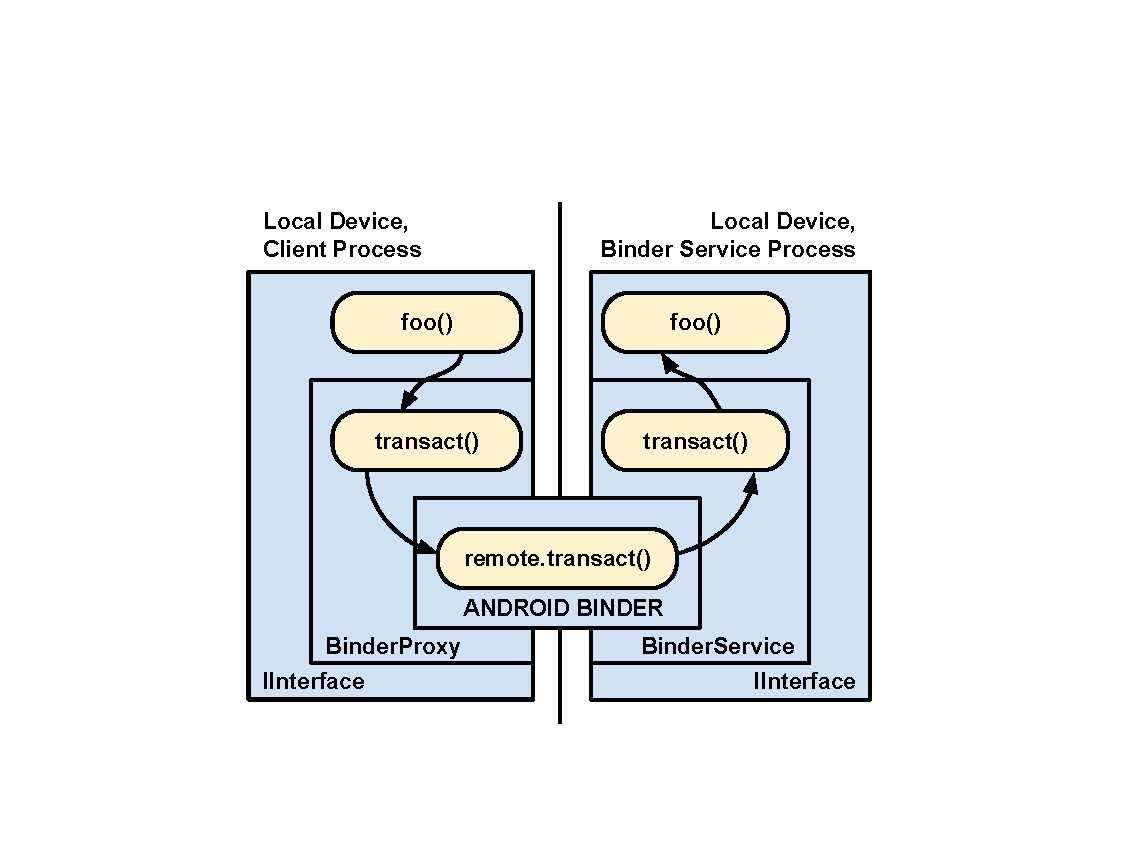
\includegraphics[width=0.3\textwidth]{drawings/proxy_pattern.pdf}
%\end{figure*}
An OO version of ServiceManager (whose service interface is provided in Appendix~\ref{app:ServiceManager}) provides the ability to register BBinder services and retrieve BpBinder proxies. An invocation of BpBinder.transact() simply invokes a binder\_call to the remote handle, and eventually invokes BBinder.transact() on the remote service process. A RPC interface is implemented on top of this structure, following a convention to implement various actions with .transact(). For instance, a FooBarService is implemented by associating each method with an ID, passed in as the code argument into .transact().

\begin{snippet}
class BpFooBarService : public BpBinder {
  void foo(int a, int b) { /* ... */ transact(1, encoded_args, ...); }
  void bar(string c) { /* ... */ transact(2, encoded_args, ...); }
  /* transact() invokes BBFooBarService.transact() on remote process
     via binder. Waits for and returns reply parcel. */
}
class BBFooBarService : public BBinder {
  void foo(int a, int b) { /* Do something useful */ }
  void bar(string c) { /* Another useful fucntion */ }
  void transact(code, msg, reply, flags) {
    switch(code) {
      case 1: /* decode args... */ foo(args); break;
      case 2: /* decode args... */ bar(args); break;
}}}
\end{snippet}

The creation of binder RPC involves boilerplate code. To make this more convenient, the Android SDK defines a domain-specific language named AIDL to specify interfaces for binder services in a language similar to the language for specifying Java interfaces. The AIDL compiler generate Stub and Proxy classes that implement the specified interface and encapsulate Binder and BinderProxy objects, respectively. A developer simply extends the Stub class, providing an implementation for each service method (like foo() and bar() above). The generated classes do all the necessary work to marshall and unmarshall arguments as Parcels and invoke the appropriate method on the actual service object. For instance, here is the AIDL definition of the FooBarService.

\begin{snippet}
interface FooBarService { void foo(int a, int b); void bar(String c); }
\end{snippet}

A binder object implementing a specified service interface can be created simply by extending the Stub class, and providing an implementation for service methods. Remote processes receive a Proxy version of the service.

\begin{snippet}
IBinder localBinder = new FooBarService.Stub() { void foo(...) { ... }
                                                 void bar(...) { ... } };
\end{snippet}

\subsection{Accessing Binder Services}
The Android Runtime provides pathways for components to communicate binder objects between each other. For instance, Android apps can declare a Service component that other components, like GUI-based Activity components, can bind to. Binding to a service brings up the Service and then returns the result of invoking its onBind() method back to the Activity. The Service returns a real instantiation of a service (i.e. an object extending the Binder class), and the Android Runtime and OO Binder framework take care to return to the Activity a BinderProxy instantiated with a remote handle to that Binder object. This assumes the Service and Activity components run as separate processes.

\begin{snippet}
class FooBarAndroidService extends Service {
  public void onBind() { return new FooBarService.Stub() { ... }; }
}

class FooBarClient extends Activity {
  public void onStart() { bindService(/* name of the service */,
                                      /* callback on connected */ this);
  }
  public void onServiceConnected(
    Context context, IBinder binder) {
    // The binder here is a BinderProxy, not the original Binder object.
    FooBarService.asInterface(binder).foo(1, 3);  // invokes RPC.
  }
}
\end{snippet}

From the point of view of the developer, it doesn't matter if the returned object is a Binder or BinderProxy. Both implement the IBinder interface, and both can be cast as the FooBarService interface. The process of retrieving a service is an easy-to-understand, asynchronous operation for the developer. However, there are a few core services of the Android Runtime that come into play to make it happen. The process is visualized in figure~\ref{fig:BindService} and detailed below.

\begin{figure}[h]
\centering
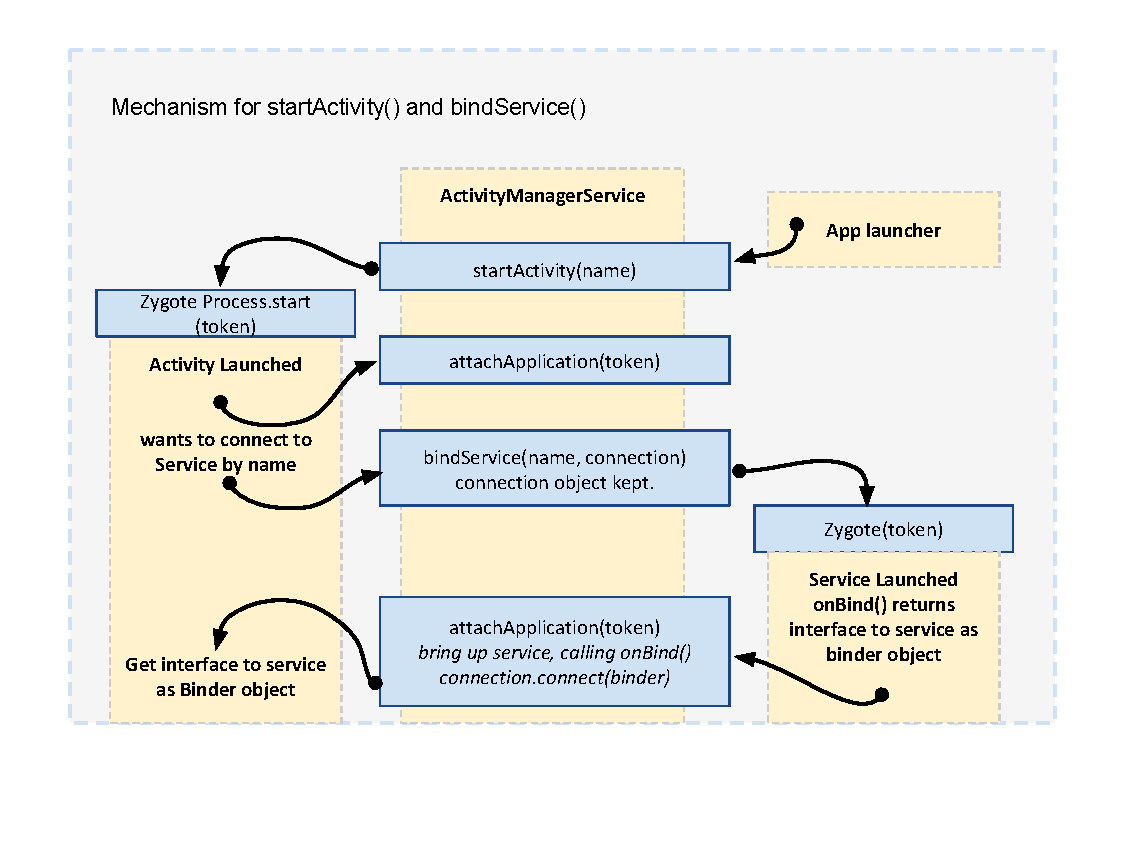
\includegraphics[width=0.85\textwidth]{drawings/bindService.pdf}
\caption{Android Runtime and Components Interaction after a bindService() RPC}
\label{fig:BindService}
\end{figure}

bindService(...) is invoked with a callback binder object--the ServiceConnection. Once the requested service is up, the ServiceConnection callback is invoked asynchronously with the requested binder service as an IBinder object. The ActivityManager works together with other essential system services to bring up and connect to the specified service component. The PackageManager, which tracks all installed components on the system, validates that the requested service component exists and checks that the caller has permissions to connect to it. If the requested service resides in a separate java package namespace, a low-level component known as Zygote brings up the service as a separate process. When the service is up, it attaches to the ActivityManager via RPC. Afterwards, ActivityManager retrieves the binder service provided by the service component as an IBinder object, and passes it on the caller by invoking the ServiceConnection callback. There are quite a few RPCs involved in this procedure!

\subsubsection{Accessing Android System Services}
bindService(...) cannot be used for everything. For instance, in the course of binding to a service, the ActivityManager brings up the service first and waits for it to attach. The newly-up service cannot use bindService() to get a reference to the ActivityManager, as that is a circular dependence. Instead core system services like ActivityManager are all available through the ServiceManager--the BKM's default context manager. It is straightforward to obtain a reference to the ServiceManager from any process or thread (i.e. make binder\_call with target=(void*)0). So it follows that it is always possible to retrieve IBinder references to any currently active service published to the ServiceManager.

\section{System Services: Provided Over the Network?}
\label{sec:SystemServices}
Before going into the design and implementation of Sigma, it is useful to understand the kinds of system services offered via binder. This will serve as guide to figure which features of binder are commonly used, and will set a baseline for the features Sigma should support. In particular, we want to answer: which services are useful for remote devices to access? And which cannot be accessed (or don't make any sense to provide access to)?  To start, it is reasonable to expose ServiceManager since it is an entry-point into all other system services. There are dozens of system services, but the patterns used repeat. So, four interesting services are covered here.

\subsection{LocationManager: location updates via binder callback and PendingIntent}
It is most natural to expose system services that are standalone and isolated in a sense. A good example is the LocationManager which ``allows applications to obtain periodic updates of the device's geographical location, or to fire an application-specific Intent when the device enters the proximity of a given geographical location.~\cite{LocationManagerDocs}'' The location manager operates as a standalone source of location updates. Here are 2 methods of the LocationManager that we look into further.

\begin{snippet}
interface ILocationManager {
  void requestLocationUpdates(
      in LocationRequest request,
      in ILocationListener listener,
      in PendingIntent intent,
      String packageName);

  void removeUpdates(
      in ILocationListener listener,
      in PendingIntent intent,
      String packageName);
  // ... among other methods
}
\end{snippet}

\begin{snippet}
oneway interface ILocationListener {
    void onLocationChanged(in Location location);
    // ... among other callback methods
}
\end{snippet}

The main requestLocationUpdates() method requires the client to provide either a ILocationListener binder callback or PendingIntent callback. If the former callback is provided, LocationManager holds a BinderProxy initialized with the remote handle to the client-provided ILocationListener. The .onLocationChanged() RPC is invoked periodically with location updates, provided that the client application keeps the callback object alive (i.e. a keep around a strong reference) and that the client process remain running.

The latter PendingIntent callback is also implemented via binder. However the callback object is managed by the Android Runtime. The client first obtains a PendingIntent via RPC to the central ActivityManager. A PendingIntent is constructed with the address of a recipient component to which messages are delivered. Used as a callback, the PendingIntent is usually constructed with the address of a component in the client's namespace (or the client component itself). With the PendingIntent provided as argument to requestLocationUpdates(), the LocationManager later can invoke PendingIntent.send() with location updates as contained data. This RPC goes to the Android Runtime (the owner of the PendingIntent), which then via another RPC routes the message to the recipient component. Though the PendingIntent mechanism is inherently more complex, the advantage is that the Android Runtime takes care to brings up the recipient component in case it is not already up. This way an app can register a PendingIntent callback and not have the burden of being active to receive callbacks.

\begin{snippet}
interface IIntentSender {
  int send(
    /* The message */
    int code, in Intent intent,
    /* Address of recipient */
    String resolvedType,
    /* Send finished callback */
    IIntentReceiver finishedReceiver,
    ...);
}
\end{snippet}

\begin{snippet}
oneway interface IIntentReceiver {
  void performReceive(
      in Intent intent, int resultCode,
      ...);
}
\end{snippet}

PendingIntent.send() is implemented in non-blocking fashion. Internally a PendingIntent is an IIntentSender binder object which is owned by (and thus invoked RPCs runs within) the ActivityManager. An additional IIntentReceiver callback can optionally be passed in with each invocation of .send()--a callback which is invoked once the send operation is complete. This additional callback is useful, as the LocationManager uses it to keep track of pending .send() operations, keeping a ``WakeLock'' while there are pending operations. A WakeLock is an Android Runtime feature that is acquired to prevent the device from entering sleep mode. Without the WakeLock, pending messages can become stuck in-flight if the device enters sleep.

Both direct binder object callbacks and PendingIntent callbacks should be supported by Sigma. PendingIntent callbacks are of particular interest since they can be used in the design of ``push'' services~\cite{PushTechnology}. With Sigma, a client can register a PendingIntent with a remote service (provided by a remote device). The client app can receive callbacks from the remote device without the need for the client app to remain active. Of course, the Sigma network stack in charge of receiving binder messages (resident on both the local and remote devices), and the service on the remote device have to be remain active for this to work.

\subsection{SensorManager: sensor events via Unix domain sockets}
The SensorManager is another good candidate to allow access from remote devices. It is a standalone source of sensor data streams. Recently, sensors services have evolved to to provide the user's activity state--e.g. categories like walking or driving~\cite{AndroidActivityRecognition}. We imagine future system services will include an variety of contextual inferences derived from sensor data.

Also interesting is SensorEvents are sent via a BitTube--an OO abstraction on top of Unix domain sockets. This mechanism is different from the binder-callback mechanism used by LocationManager. Here, SensorManager uses binder to setup a unix domain socket pair between two processes, and subsequently pushes sensor events over the socket. If we are to expose SensorManager over the network, we need to the ability to send file descriptors (and importantly: to support IO operations on those file descriptors) over the network as well.

\begin{snippet}
class ISensorServer : public IInterface {
public:
    Vector<Sensor> getSensorList() = 0;
    sp<ISensorEventConnection>
      createSensorEventConnection()
    // ... among other methods
};
\end{snippet}

\begin{snippet}
class ISensorEventConnection : public IInterface {
public:
    sp<BitTube> getSensorChannel()
    status_t enableDisable(int handle, bool enabled)
    status_t setEventRate(int handle, nsecs_t ns)
};
\end{snippet}

\subsection{AlarmManager: not very useful over the network}
There are some services which don't make too much sense to expose. For instance, the AlarmManager is intended for cases where you want to have application code run at a specific time. It works via PendingIntent callbacks that serve as alarms to wake up a process for scheduled execution. There is no need to access a remote device's alarm manager as it provides no useful data or service more than that provided by the local instance of AlarmManager.

\subsection{ActivityManager: difficult to expose over network without extensive refactoring}
Services that are coupled to the local Android Runtime are difficult to directly expose over the network. This is because the operation of such services depends on records that are local to the device. For instance, ActivityManager is a crucial system service that is in charge of managing all live components running on the Android device. All components attach to the ActvityManager when they run, and through the ActivityManager provide useful operations such as bindService(). However, it is not so straightforward to invoke bindService() on a remote handle to ActivityManager (running on a different device). Such a RPC refers to records about the calling process that only the ActivityManager on the client device knows about.

\subsection{A caveat with Android Permissions}
A complication, particularly when dealing with system services, is that many of them require permission to access. Apps declare permission to use a service, and the PackageManager grants such permission at install time. It is not trivial to extend the Android permissions system to allow access system services on remote devices. As such Sigma as it is implemented disregards Android permissions, allowing apps to access to all services running on a remote device. A thorough treatment of the permissions framework and its support by Sigma is a left for future work, with discussion at the end of the paper in Sections~\ref{sec:DealingWithAndroidPermissions} and ~\ref{sec:NextSteps}.

\section{Sigma: Design and Implementation}
\label{sec:Sigma}
\begin{figure}[h]
\centering
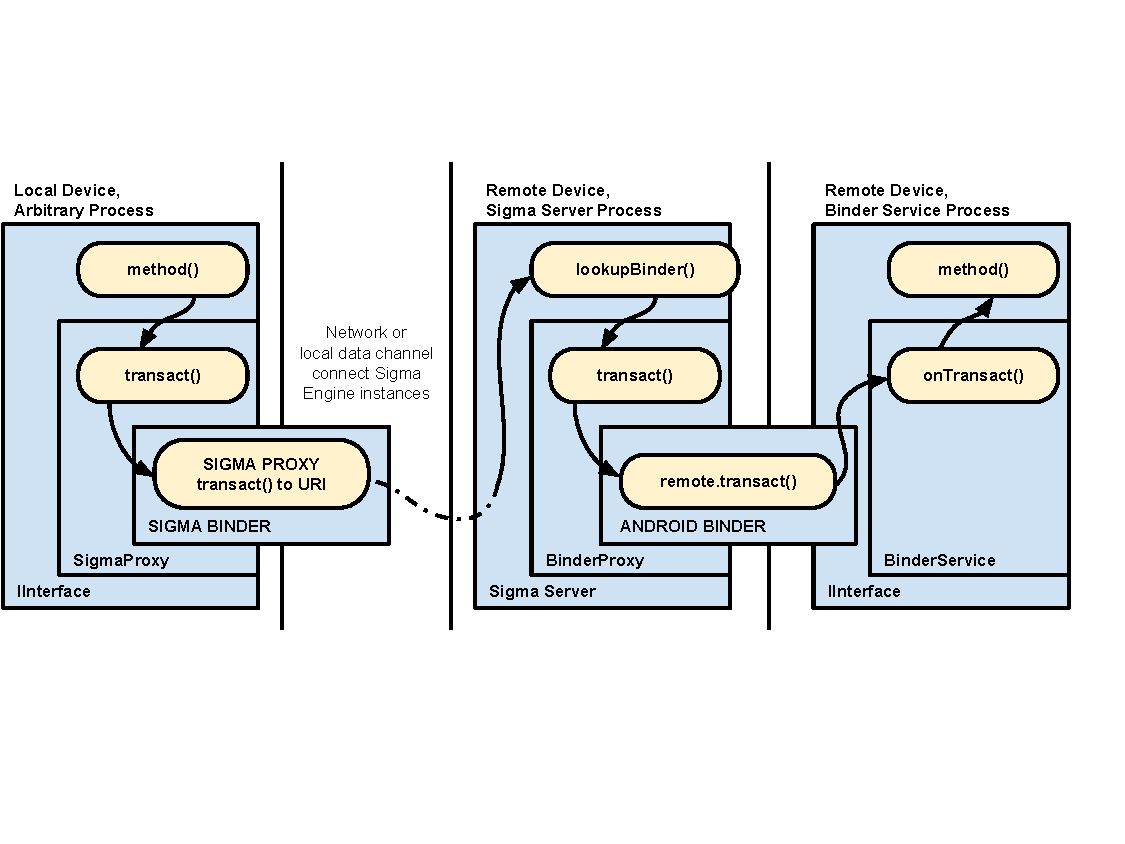
\includegraphics[width=0.8\textwidth]{drawings/sigma_proxy_pattern.pdf}
\caption{Sigma as a chained Proxy Pattern}
\label{fig:SigmaChainProxy}
\end{figure}
The design of Sigma in a nutshell is essentially to follow the Proxy Pattern of binder services one hop out--with a ``Proxy'' Binder on a client device forwarding all operations to a remotely managed IBinder object on another device, see figure~\ref{fig:SigmaChainProxy}. We are mainly interested in supporting .transact(), and that entails the communication of Parcel objects from one device to another.

%\textbf{Caveat} As Sigma is implemented today, it requires some underlying modifications to the Android Runtime, as such it is not compatible with regular Android devices. See Appendix~\ref{sec:AndroidRuntimeModifications}

Consider a network consisting of two Android devices, and that there is a pre-established data channel between them. Each device runs a Sigma Engine instance which has server-like and client-like functions. Its function viewed as a server is to associate a URI to a local IBinder object given to it--usually a BinderProxy object referring to an active Binder object running on another process on the same device. Subsequently Sigma Engine should listen on the network channel for requests made to that URI, and perform the requested operation directly on the corresponding managed IBinder object. Its function as a client is to communicate over the network channel with a remote Sigma Engine to retrieve the URI of a remotely managed IBinder object. The local Sigma Engine then creates a special Binder object--a SigmaProxy which is initialized with the URI of the remotely managed IBinder. A handle to SigmaProxy can be passed to other processes on the local device, as a BinderProxy object. Local clients can invoke .transact() on the SigmaProxy via binder. This operation runs on the Sigma Engine (as it created the SigmaProxy) and it functions to forward the binder transaction (its arguments) to the remote Sigma Engine--invoking its server-like functions--to handle the binder transaction, and eventually return a reply.

\subsection{Dealing with Binder Objects in a Parcel}
The difficulty arises when dealing with the contents of the Parcel arguments in a call to .transact(). Since a Parcel can contain handles to local binder objects or file descriptors, we cannot simply marshall the Parcel's byte-array and expect the the unmarshalled Parcel to be valid on the remote side.

When .transact() is invoked on a SigmaProxy, the ``msg'' Parcel object needs to be communicated over the network channel. However, the Parcel may contain local descriptors such as handles to binder objects. With some modifications to the Android Runtime (see Appendix~\ref{sec:AndroidRuntimeModifications}), we are able to locate the offsets into the Parcel's byte-array where these handles are written, and are able to read in each handle as a BinderProxy object. We now utilize the server-like functions of the Sigma Engine by asking it to manage each BinderProxy object--assigning it an URI. Thus, each Parcel containing handles to binder objects are rewritten into messages containing the corresponding URIs. Each URI is managed by the Sigma Engine. See the encode side of figure~\ref{fig:encodeParcel}.

On the remote end, the Sigma Engine receives a binder transaction request targeted to a URI of an IBinder object that it manages. The request contains an encoded Parcel with an array of URIs (pointing to an IBinder managed by a Sigma Engine on another device). Utilizing the client-like functions of Sigma Engine, we create SigmaProxy Binder objects targeted at each URI. A Parcel object is created, writing handles to these SigmaProxy objects into the Parcel's byte-array (into the same offsets as in the original Parcel). See the decode side of figure~\ref{fig:encodeParcel}. The Sigma Engine then calls .transact() on the target IBinder with this newly created Parcel. The reverse procedure is used in returning the ``reply'' Parcel object back to the caller Sigma Engine.

\begin{figure}[h]
\centering
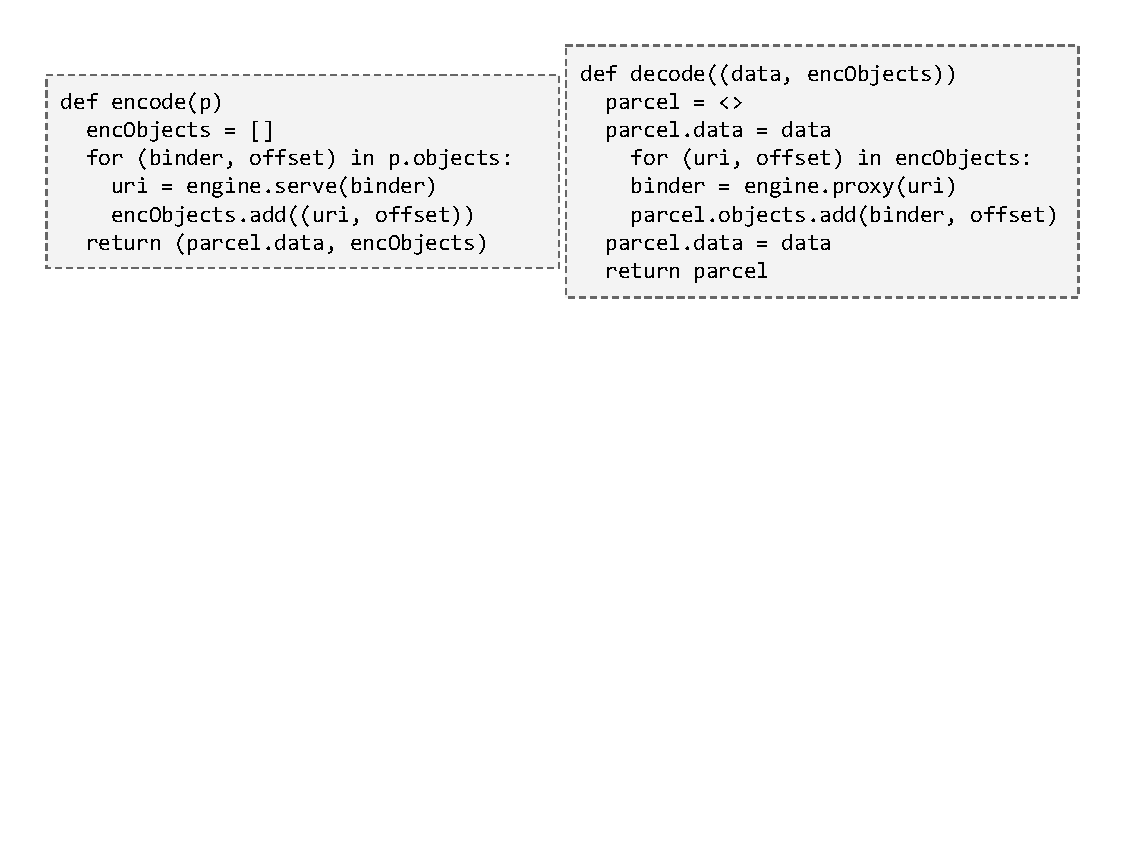
\includegraphics[width=0.8\textwidth]{drawings/encodeObjects.pdf}
\caption{Pseudo-code algorithm for encoding binder objects as URI, and creating a binder object on the other end targeted at that URI.}
\label{fig:encodeParcel}
\end{figure}

\subsubsection{Reference counting}
\label{sec:ReferenceCounting}
Another detail is reference-counting. A Binder object remains in memory as long as there is at least one strong reference to it. So, a SigmaProxy object will remain in memory unless deleted by the Sigma Engine that created it. On the other hand, a strong reference to a BinderProxy object does not prevent the referent Binder object from being garbage collected. This routinely happens, and causes a ``DeadObject'' exception when invoking a RPC on a dead referent Binder.

In the original Binder implementation, there is no additional Binder object created. As remote processes simply hold BinderProxy objects to referent Binder objects from another process. So it follows, we have to specifically handle clean-up in the implementation of Sigma. The way we manage it is to hold only a weak reference to BinderProxy objects managed by the Sigma Engine. This way, BinderProxy objects are finalized when the referent Binder dies. And when that happens, the Sigma Engine can send a message over the network channel to invalidate all remote SigmaProxy objects pointed to the URI of the finalized BinderProxy object. See the evaluation in section~\ref{sec:location_sharing} that tracks the allocation and de-allocation of Binder objects to see an example of Sigma's reference-counting mechanism at work.

\subsection{Dealing with File Descriptors in a Parcel}
File descriptors in Parcels are handled analogously to binder objects. However, in Unix-like systems, file descriptors can refer to any Unix file type named in a file system. As well as regular files, this includes directories, block and character devices (also called ``special files''), Unix domain sockets, and named pipes. File descriptors can also refer to other objects that do not normally exist in the file system, such as anonymous pipes and network sockets~\cite{UnixDomainSocket}.

Although it is theoretically possible to handle each type of file descriptor (the way Netcat~\cite{NetCatProxy} manages to be a proxy), each type has to be treated separately since each type has a specific set of supported IO operations. We only want to demonstrate as a proof-of-concept that we can handle file descriptors by focusing on a single type: the Unix domain socket. This type is interesting mainly because it is used by SensorManager to communicate sensor events, and used elsewhere in GUI-related Android services. Such file descriptors are created via socketpair() with the protocol SOCK\_SEQPACKET, and provide sequenced, reliable, bidirectional, connection-mode transmission paths for records. A record can be sent using one or more output operations and received using one or more input operations, but a single operation never transfers part of more than one record~\cite{SocketManPage}. Fortunately, we need to support only a small set of operations: send() and recv(). Also the remote end needs to know when the socket is no longer valid or is otherwise closed so that resources can be cleaned up.

Unlike a binder object where requests are unidirectional (from SigmaProxy to remotely managed IBinder), the socket is bidirectional. When a SigmaProxy handles a transaction with a unix domain socket in the Parcel, it is managed in two ways. First, the server-like part of Sigma Engine listens on the network channel for received data (which is forwarded to it from a remote Sigma Engine). When this happens, the data is sent on the managed socket. Second, a Forwarder thread is started which polls for data received by the managed socket, and forwards any data to a remote URI (where the remote Sigma Engine is already listening for data). The pseudo-code for encoding and decoding file descriptors and the pseudo-code of the Forwarder is provided in figures~\ref{fig:encodeFds} and ~\ref{fig:fdForwarder}, respectively.

\begin{figure}[h]
\centering
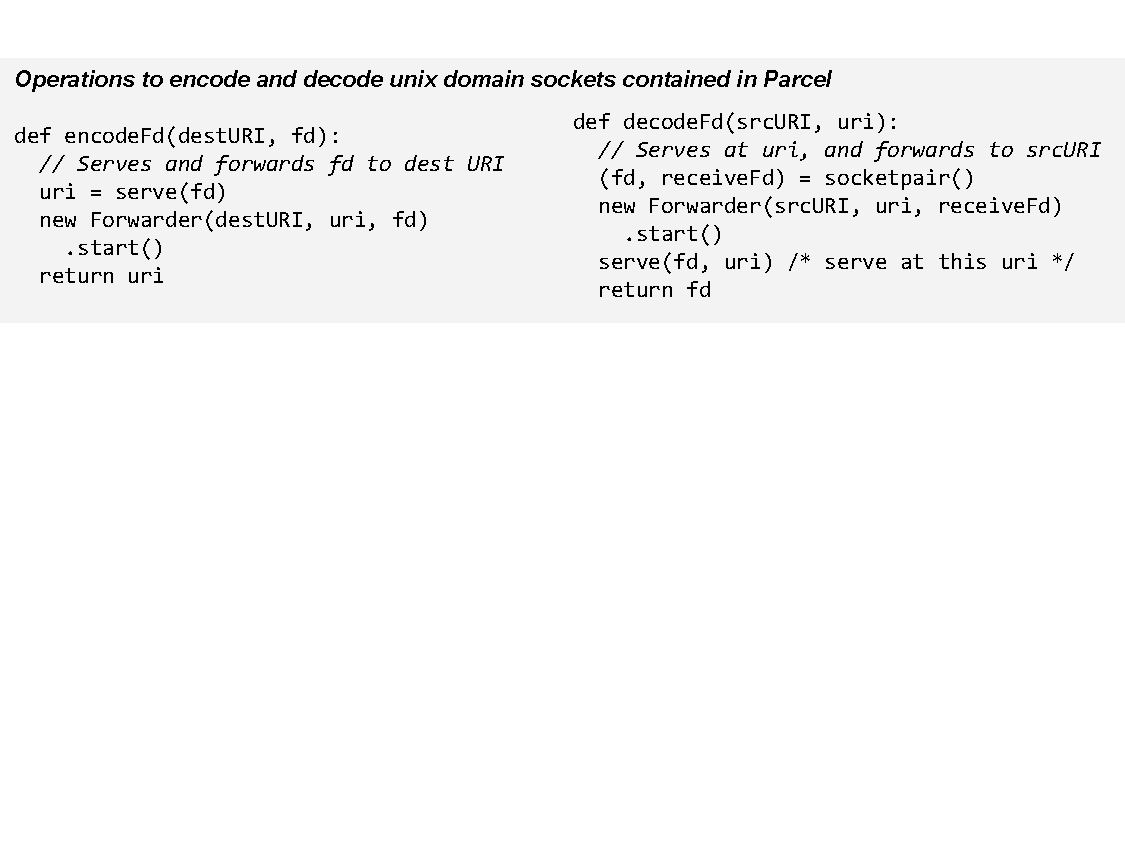
\includegraphics[width=0.8\textwidth]{drawings/encodeFds.pdf}
\caption{Pseudo-code algorithm for encoding (UNIX\_DOMAIN\_SOCKET) file descriptors as URI, and creating a new file descriptor at the other end targeted at that URI.}
\label{fig:encodeFds}
\end{figure}

\begin{figure}[h]
\centering
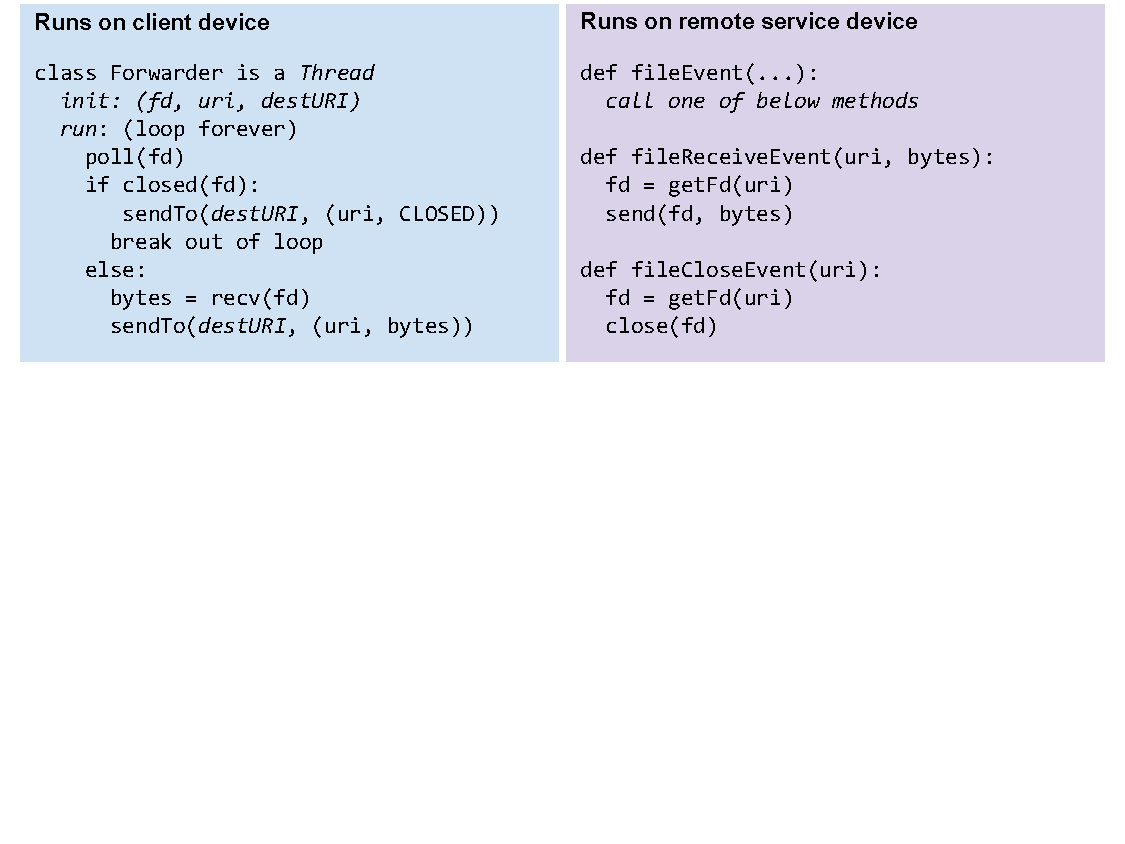
\includegraphics[width=0.8\textwidth]{drawings/forwardFds.pdf}
\caption{Pseudo-code for a file descriptor event forwarding mechanism. Polls and forwards messages received on one end towards the URI. Then messages are forwarded to the local file descriptor on the other end.}
\label{fig:fdForwarder}
\end{figure}

\subsection{Design of the Sigma Message-based Protocol}
Sigma Engine needs a networking stack to work. The first decision is about where to implement the networking stack. It makes sense to implement at the Java level--using the features of the Java Android Runtime and convenience of the Android SDK to full benefit. Particularly since we have established that Sigma itself can be implemented purely in Java with some prerequisite modifications to the Android Runtime (see Appendix~\ref{sec:AndroidRuntimeModifications}).

The second decision is to chose a structured format for communication over the network data channel. The choice is arbitrary, but we wanted something relatively fast and with the ability to define data types or schemas for messages. Our choice is a lightweight implementation of Google's protobuf format for encoding structured data called Wire~\cite{Wire,IntroWire}. It is a open source library created specifically for Android by the mobile app company Square.

A basic building block is representing a URI. It is a Wire message (see Figure~\ref{fig:WireURI}) that contains all the necessary network information about the source or target Sigma Engine. When a URI contains only that much information, it is known as a BASE URI. An HTTP-based Sigma Engine has a URI with the host and port fields set, for instance. A URI can also refer to a remotely managed IBinder object. A BINDER URI is a BASE URI (which refers to a Sigma Engine) with additional fields set: the assigned ID of the referent binder and its interface descriptor. If the binder object was originally from a Parcel, then its offset into the Parcel's byte-array is also set. Similarly, a UNIX\_DOMAIN\_SOCKET URI is a BASE URI along with the assigned ID of the managed socket file descriptor. The URI.ObjectType field distinguishes between these types of URIs.

\begin{figure}[h!]
\centering
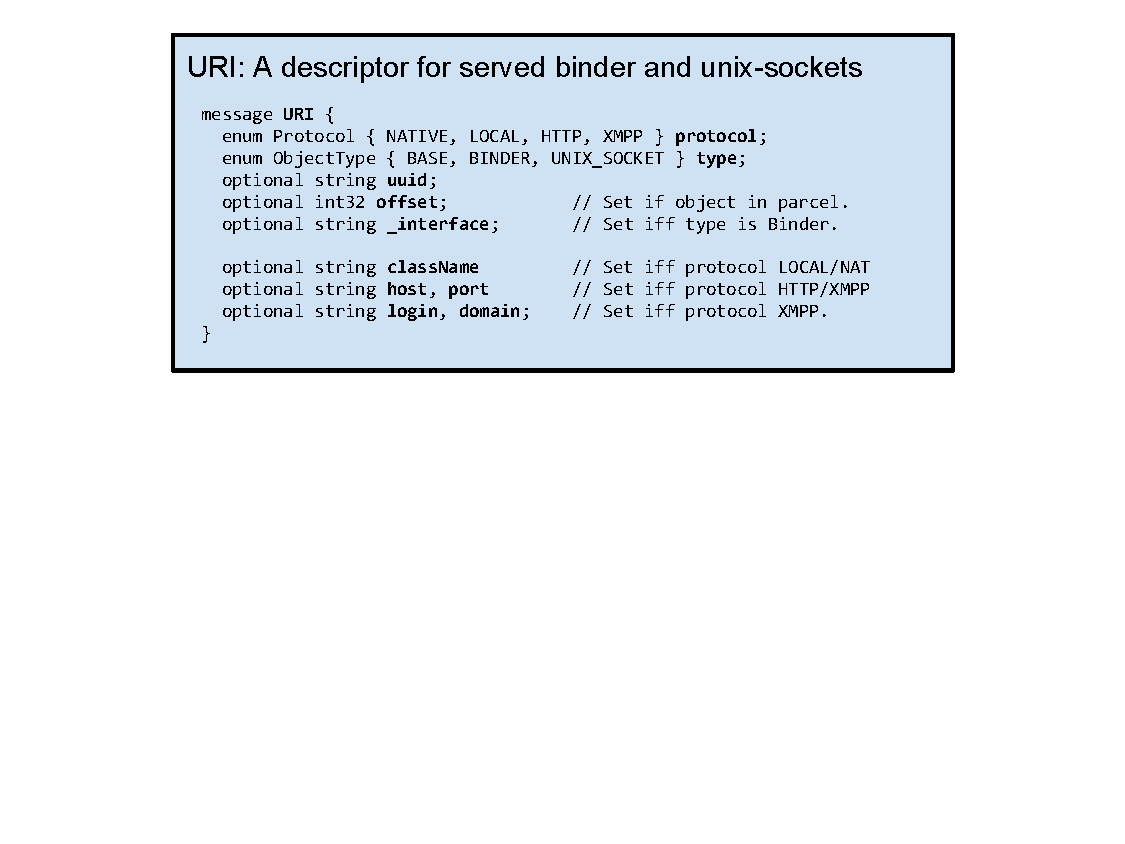
\includegraphics[width=0.8\textwidth]{drawings/WireURI.pdf}
\caption{A Wire message for representing URI for remote Sigma engines, binder objects, and file descriptors}
\label{fig:WireURI}
\end{figure}

The messages exchanged between Sigma Engines is implemented in transactions, where there may be many transactions made in parallel. Each transaction is modeled with a pair of Wire messages: a SRequest message followed by a SResponse message. Figure~\ref{fig:GenericSigmaTransaction} contains the rough protobuf format implementing the basic transaction.

\begin{figure}[h!]
\centering
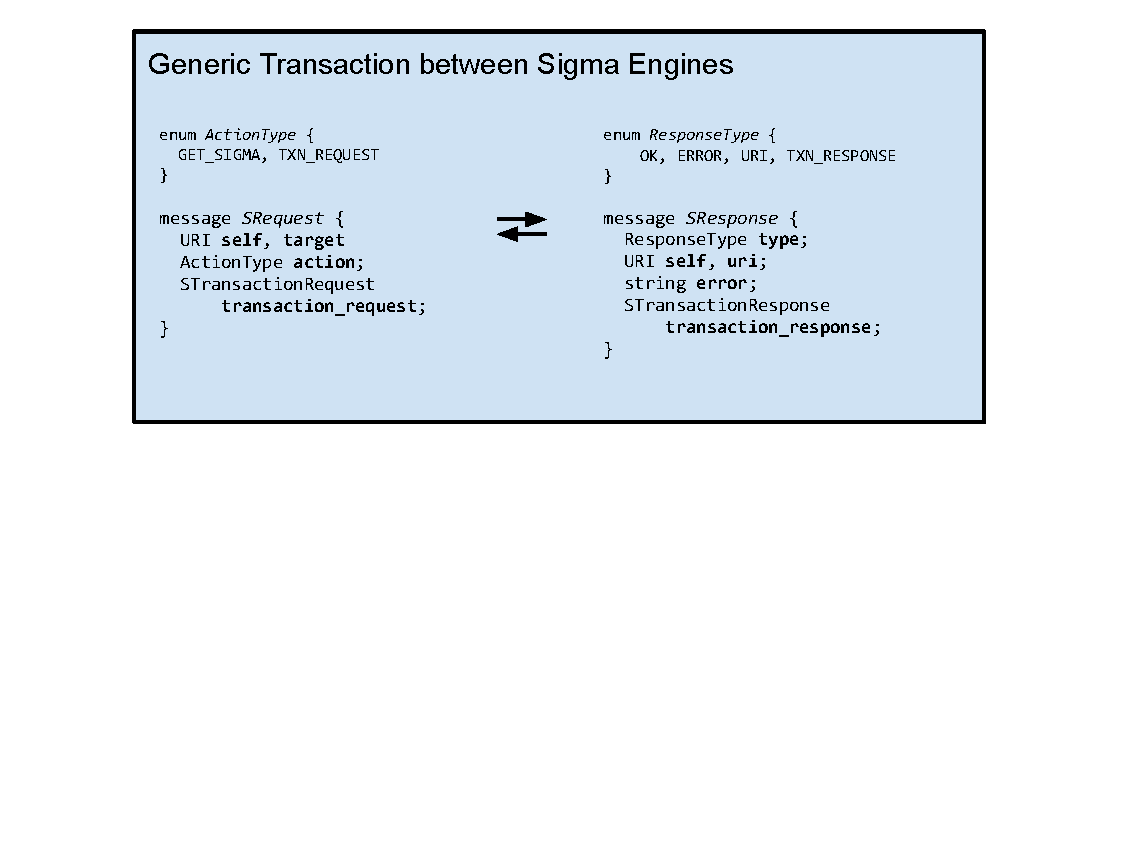
\includegraphics[width=0.8\textwidth]{drawings/WireTransaction.pdf}
\caption{Wire messages for a generic Sigma transaction}
\label{fig:GenericSigmaTransaction}
\end{figure}

There are only two types of SRequest. The GET\_SIGMA Request is the entrypoint; it is the first request made to a remote Sigma Engine. It returns a URI SResponse containing the BINDER URI of the remote Sigma Engine's very own binder service known as ISigmaManager. Further requests are binder transactions (SRequests of type TXN\_REQUEST) made to the ISigmaManager (initially) or to other BINDER URIs managed by the remote Sigma Engine. Much like the ServiceManager is the entrypoint to retrieve local binder services, the ISigmaManager is the entrypoint to remote binder services. Its service interface is described in Section~\ref{sec:SigmaAsABinderService}.

The TXN\_REQUEST SRequest message and the corresponding TXN\_RESPONSE SResponse message encapsulate an STransactionRequest and STransactionResponse message, respectively. See figure~\ref{fig:GenericSigmaBinderTransaction}. These sub-types are the primary container for performing a .transact() operation on a remotely managed IBinder object. The request and response messages both contain Parcel objects encoded as SParcel messages. SParcel messages contain the Parcel's raw byte-array encoded as a Base-64 encoded string. This is sufficient when no objects or file descriptors are contained. The SParcel additionally contains an array of URIs with the URI's offset fields set when the Parcel does contain objects or file descriptors.

\begin{figure}[h!]
\centering
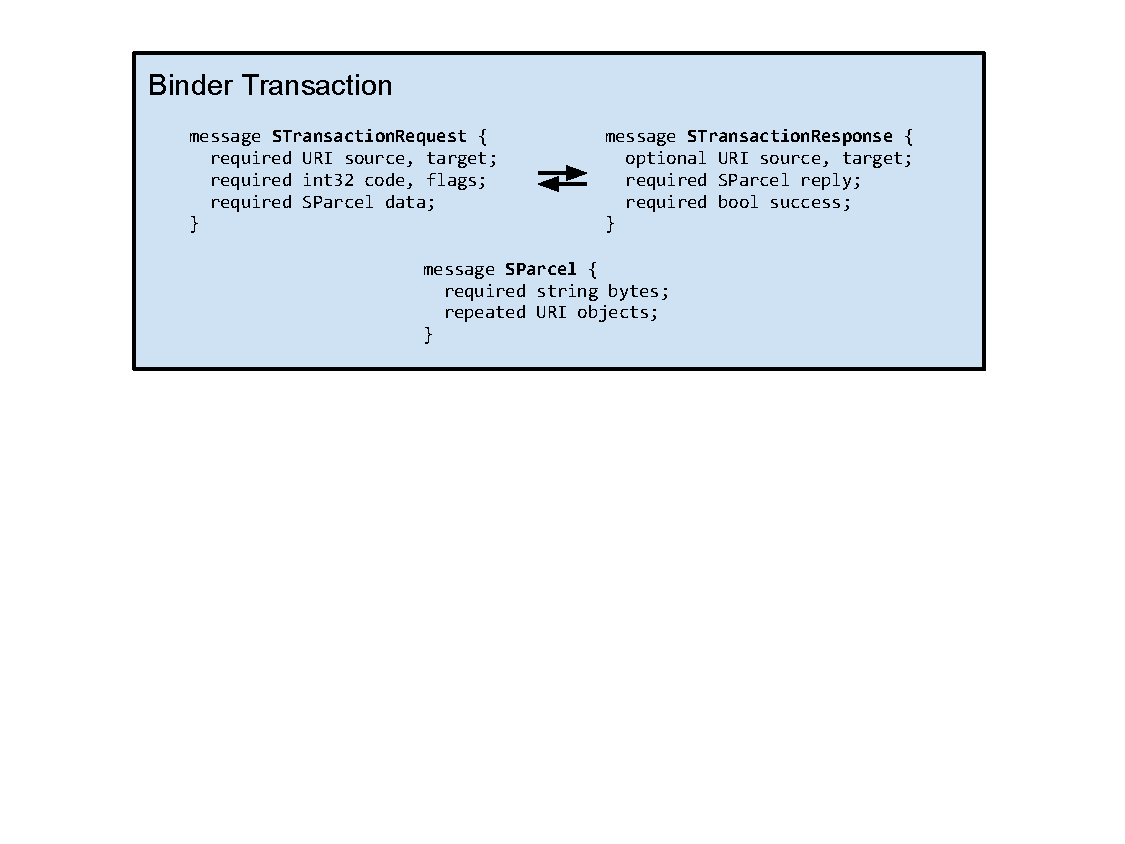
\includegraphics[width=0.8\textwidth]{drawings/WireBinderTransaction.pdf}
\caption{Wire messages for a generic Sigma binder transaction}
\label{fig:GenericSigmaBinderTransaction}
\end{figure}

\subsection{Choice of Network Data Channel}
Sigma is first a protocol and then an implementation. As a protocol, it is agnostic to the underlying network connection, assuming only that a reliable underlying data channel is available for atomically sending and receiving messages. We can evaluate and test the design of Sigma with a single Android device, simply using an IPC mechanism. To evaluate Sigma between Android devices, we have a gamut of networking technologies to choose from. We choose HTTP- and XMPP- based channel to test the design and measure performance.

\subsubsection{BINDER}
A basic version of Sigma is implemented locally using Android Binder itself as a data channel. This is useful for testing as we can run two instances of Sigma engine as separate processes on the same device. A transaction is simply a binder RPC, made from one Sigma Engine instance to another, calling a method with the following signature:

\begin{snippet}
SResponse handleRequest(SRequest request);
\end{snippet}

\subsubsection{HTTP}
Each device brings up a HTTP server listening on a pre-determined port. One device communicates to another through HTTP POST requests. One transaction corresponds to one POST request, and parallel requests may be made if supported by the server. To establish a data channel, one device needs to know the hostname and port of the other device, and the other device's HTTP server must be accessible over the network.

\subsubsection{XMPP}
Each device logs-in with a distinct alias to a mutually accessible XMPP server. XMPP is a popular protocol for real-time collaboration--messaging and chat. Transactions initiate a chat session with another active alias. Each chat session, identified by a unique thread ID, is used for one transaction and then disposed. Subsequent (or parallel) transactions occur on distinct sessions.

\subsubsection{Encoding Wire Messages, Examples}
The Sigma Engine creates Wire messages for each transaction. These can be printed to human-readable format. For instance, here is a BIDNER URI for a ICommentReceiver (IBinder) object managed by a XMPP-based SigmaEngine that is using the alias ``rr@quark.''

\begin{snippet}
URI{_interface=com.example.BinderSigma.samples.chat.ICommentReceiver,
domain=quark, login=rr, protocol=XMPP, type=BINDER,
uuid=c2f980b5-ae50-4f7e-9559-438abc49508f}
\end{snippet}

Such Wire messages are compactly serialized into byte arrays. Over HTTP, the byte array is sent directly via a POST request as a byte-array entity. Over XMPP, the byte array is first made into a Base64-encoded string and then sent as a chat message. Below is an example of a SRequest sent as an XMPP chat message (note: the SRequest is serialized then Base64-encoded)

\begin{snippet}
<message type="chat" id="30e5a4c7-b0d7-4d11-bd2c-14abf4ff1ce0"
        to="kk@quark" from="rr@quark/Smack" >
        <body> <!-- Base-64 encoded string --> </body>
        <thread>877a1f <!-- id of transaction --> </thread>
        </message>
\end{snippet}

Appendix sections~\ref{app:WireExchange} and ~\ref{app:WireExchangeRecursive} contain example exchanges of Wire messages between two Sigma Engines.

\subsection{The ISigmaManager entrypoint to remote binder services}
\label{sec:SigmaAsABinderService}
The Sigma Engine is implemented as an Android service component. It is brought up with a BASE URI that serves as the Sigma Engine's identity going forward. There are separate Android Service Components for each implementation (i.e. one for the LOCAL, HTTP, and XMPP implementations). Bringing up one such implementation and binding to it returns a remarkably simple service interface. This is the interface which can be used by app developers to get remote services as IBinder objects.

\begin{snippet}
interface ISigmaManager {
    URI getBaseURI();
    ISigmaManager getRemoteManager(in URI targetBaseURI);
    IBinder getServiceManager();
    /* synchronous version of bindService(Intent...) */
    IBinder getService(in Intent intent);
}
\end{snippet}

Consider an example. Assume that there are two distinct sigma engine instances, $\Sigma$A and $\Sigma$B, running on two devices, named A and B respectively. An app can access its own local Sigma Engine instance and make use of the provided ISigmaManager service. The following pseudo-code walks through the steps taken by an app running on device A to bring up and access a remote service installed on device B. It is assumed $\Sigma$B is already up and running, listening for connections.

\begin{snippet}
sigmaManA = connectToLocalSigmaEngine($\Sigma$A) /* via normal Android Runtime bindService(..) */
sigmaManB = sigmaManA.getRemoteManager(uriB) /*  Assume the URI to $\Sigma$B is already known */
remoteBinder = sigmaManB.getService("com.example.FooBarService");
remoteBinder.foo() /* Invoke remote binder's .transact(), goes through SigmaProxy */
\end{snippet}

To get a sense of the interaction between the processes on the two devices, figure~\ref{fig:SigmaInteraction} is a useful visualization. It follows the first 3 lines from above (and does not show the .foo() call).

\begin{figure}[h]
\centering
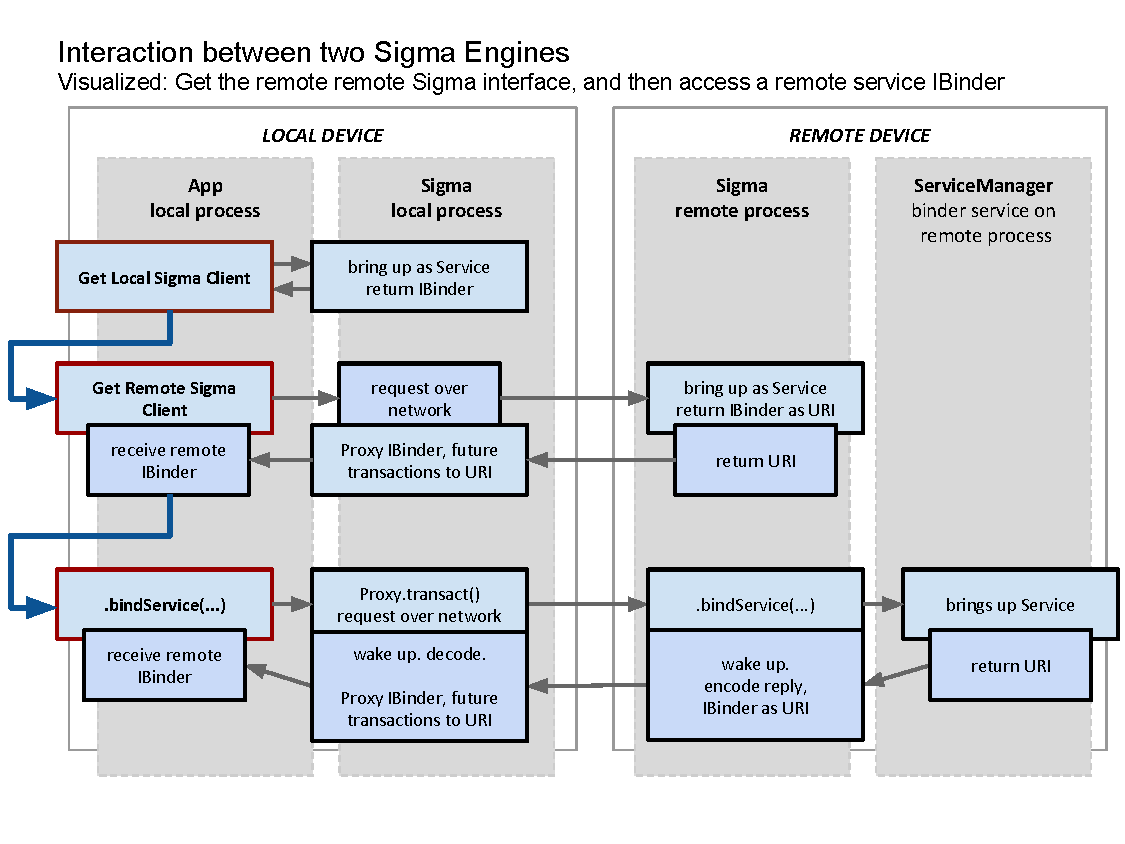
\includegraphics[width=0.8\textwidth]{drawings/SigmaEngineInteraction.pdf}
\caption{Interaction between two Sigma Engine instances for a local client to obtain an IBinder reference to a remote service.}
\label{fig:SigmaInteraction}
\end{figure}

\subsection{Accessing remote system services}
As we know, all system services are published to the ServiceManager. ISigmaManager allows access to this entrypoint via the .getServiceManager() method, enabling a client app on one device to access system services from another. However, the remote service interface is usually not the interface used by client apps. Often the remote interface is wrapped up in local client object that provides the actual service to clients, managing communication to a remote service internally. To alleviate this issue, Sigma provides a convenient RemoteContext class that is constructed with reference to a remote ServiceManager. It provides a getSystemService(name) method that implements code to retrieve remote system services and wraps them up in a client object that is more usable.

As a proof-of-concept we have implemented the retrieval of two remote services--the LocationManager and SensorManager. Many services are easily wrapped in local client objects. The local LocationManger client is straightforward to construct using reflection from the internal ILocationManager service. However, SensorService (the internal binder service providing sensor events) has a local client with parts implemented in C++ and other parts in Java (via JNI). Further complicating matters, the SensorManager is hard-coded to retrieve only the local SensorService! So it is impossible via reflection or other hacks to construct a SensorManager client with a remote SensorService handle. To enable this, we had to modify the Android runtime--the source code is available online, the link is found in Appendix~\ref{app:SourceCode}.


\section{Performance Evaluation}
\label{sec:Performance}
It is useful to know the CPU cost and latency to establish a proxy to a remote binder service and then the cost to make RPCs on that proxy. Overhead is expected due to the additional IPC within each device (there is communication from apps and services to the Sigma Engine). There is also the cost of encoding/decoding parcels during binder transactions, of creating requests and response messages, and naturally there is some cost to network IO. We first describe some simple test binder services and then present the execution timing for invoking RPCs on these test services.

\subsection{Testing Simple Binder Services}
As a first test, consider a trivial binder service: a random number server. The implementation (and implied interface) is below.

\begin{snippet}
class RandomServer extends IRandomServer.Stub() {
  int getRandom() { return (new Random()).nextInt(); }}
\end{snippet}

As a second test, consider a binder service that accepts binder object arguments. In particular, using this feature it is possible to specify a callback object that invokes a another binder transaction back to the caller device. Taking it one step further, recursion can occur back-and-forth as a series of binder calls between the two devices. The following binder service called PingPongService implements such a test. We can invoke a recursive case by a call like: remote.ping(local, 10), where both remote and local are instances of IPingPongServer, each on a different device. This causes a cascade of recursive calls, each counting down the number argument.

\begin{snippet}
class PingPongService extends
    IPingPongService.Stub() {
  void ping(IPingPongService other, int count) {
    if (count > 0) other.pong(this, count - 1);
  }
  void pong(IPingPongService other, int count) {
    if (count > 0) other.ping(this, count - 1);
  }
}
\end{snippet}

\subsection{Performance Measurements}


\begin{figure}[h]
\centering
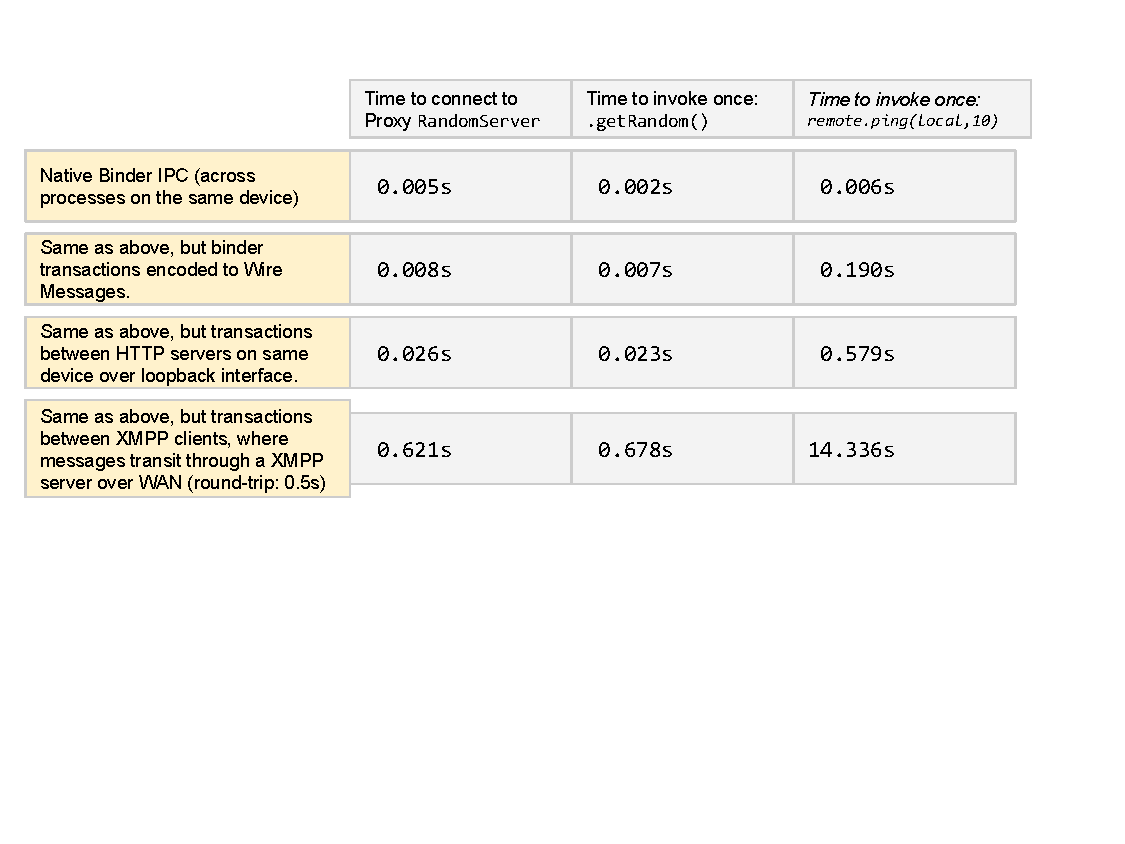
\includegraphics[width=0.85\textwidth]{drawings/Performance.pdf}
\caption{Execution timing of various binder RPC using Sigma, see section~\ref{sec:Performance} for evaluation setup}
\label{fig:performance}
\end{figure}

The result of timing various RPCs, from the services above, is plotted in figure~\ref{fig:performance}. These are timed for 3 prototype implementations each using a different type of data channel for communication. These results were obtained by running Sigma on a Nexus 4 (and emulator running on a PC, where applicable). The underlying Android Runtime is a custom version incorporating the modifications discussed in Appendix~\ref{sec:AndroidRuntimeModifications}.

As is apparent, it is 2x-3x as expensive to perform a binder call over a proxy that encodes messages than it is to make a straight, native binder call. However, the recursive PingPong test is quite expensive since each recursive call is a new binder transaction with another round of encoding and decoding, with added network overhead.

\subsection{Testing Performance with System Services}

The following assumes knowledge of the respective system services, a overview of which was previously provided in section~\ref{sec:SystemServices}.

\subsubsection{Remote Location Updates}
\label{sec:location_sharing}
We demonstrate that location updates can be requested from a remote device. As we have already demonstrated that binder object callbacks are supported by Sigma (see the above PingPong example), in this test we request location updates with the PendingIntent approach.

We have implemented the demonstration with location updates streamed from a real device (a Nexus 4) to an emulator running on a PC both on the same LAN. The data channel is an XMPP-based channel, with a central XMPP server located on the internet (in Amazon EC2 cloud, with a large round-trip time from LAN to cloud of ~500ms). Both devices login with distinct aliases into the same XMPP server. The interaction diagram in figure~\ref{fig:LocationUpdateInteraction} details the binder objects shared with between the Nexus 4 and emulator.

\begin{figure}[h]
\centering
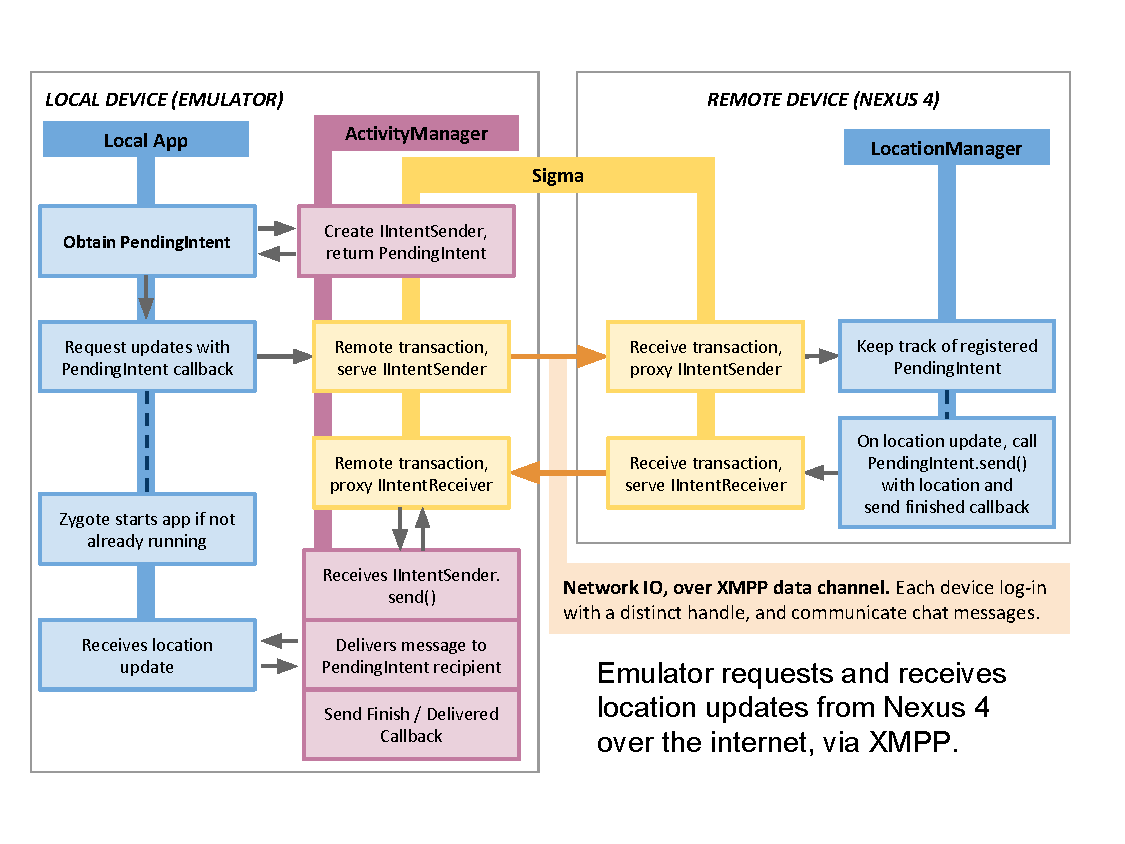
\includegraphics[width=0.7\textwidth]{drawings/LocationPendingIntentExample.pdf}
\caption{Interaction between Emulator and Nexus 4, as Emulator sets up and receives location updates from Nexus 4 via PendingIntent messages.}
\label{fig:LocationUpdateInteraction}
\end{figure}

Useful metrics to measure include CPU load and memory usage. The CPU usage of Sigma actively encoding messages and sending them over XMPP is measured at a reasonable average CPU utilization of ~10\%--measured using the dumpsys command provided by Android. Memory usage is more interesting. We can track heap allocation and separately track the number of Binder objects and Proxy objects allocated by each process--also through the dumpsys command. Remarkably, this is a good way to test and evaluate Sigma's reference counting mechanism detailed in section~\ref{sec:ReferenceCounting}. Since location updates are sent with via the PendingIntent.send() method, each send operation creates a new ``send finished'' callback--an IIntentReceiver object. Each such object is a Binder owned by the Android Runtime on the Nexus 4, and managed by its Sigma Engine. On the emulator, corresponding SigmaProxy objects are created targeted at the remote IIntentReceivers. As IIntentReceiver Binders (and associated BinderProxies) are finalized on the Nexus 4, the implemented reference-counting system nulls out the corresponding SigmaProxy objects on the emulator. Then garbage collection on emulator finalizes these over time. The allocation and deallocation of Binder objects between the two devices is visualized in figure~\ref{fig:reference_counting}.

\begin{figure}[h]
\centering
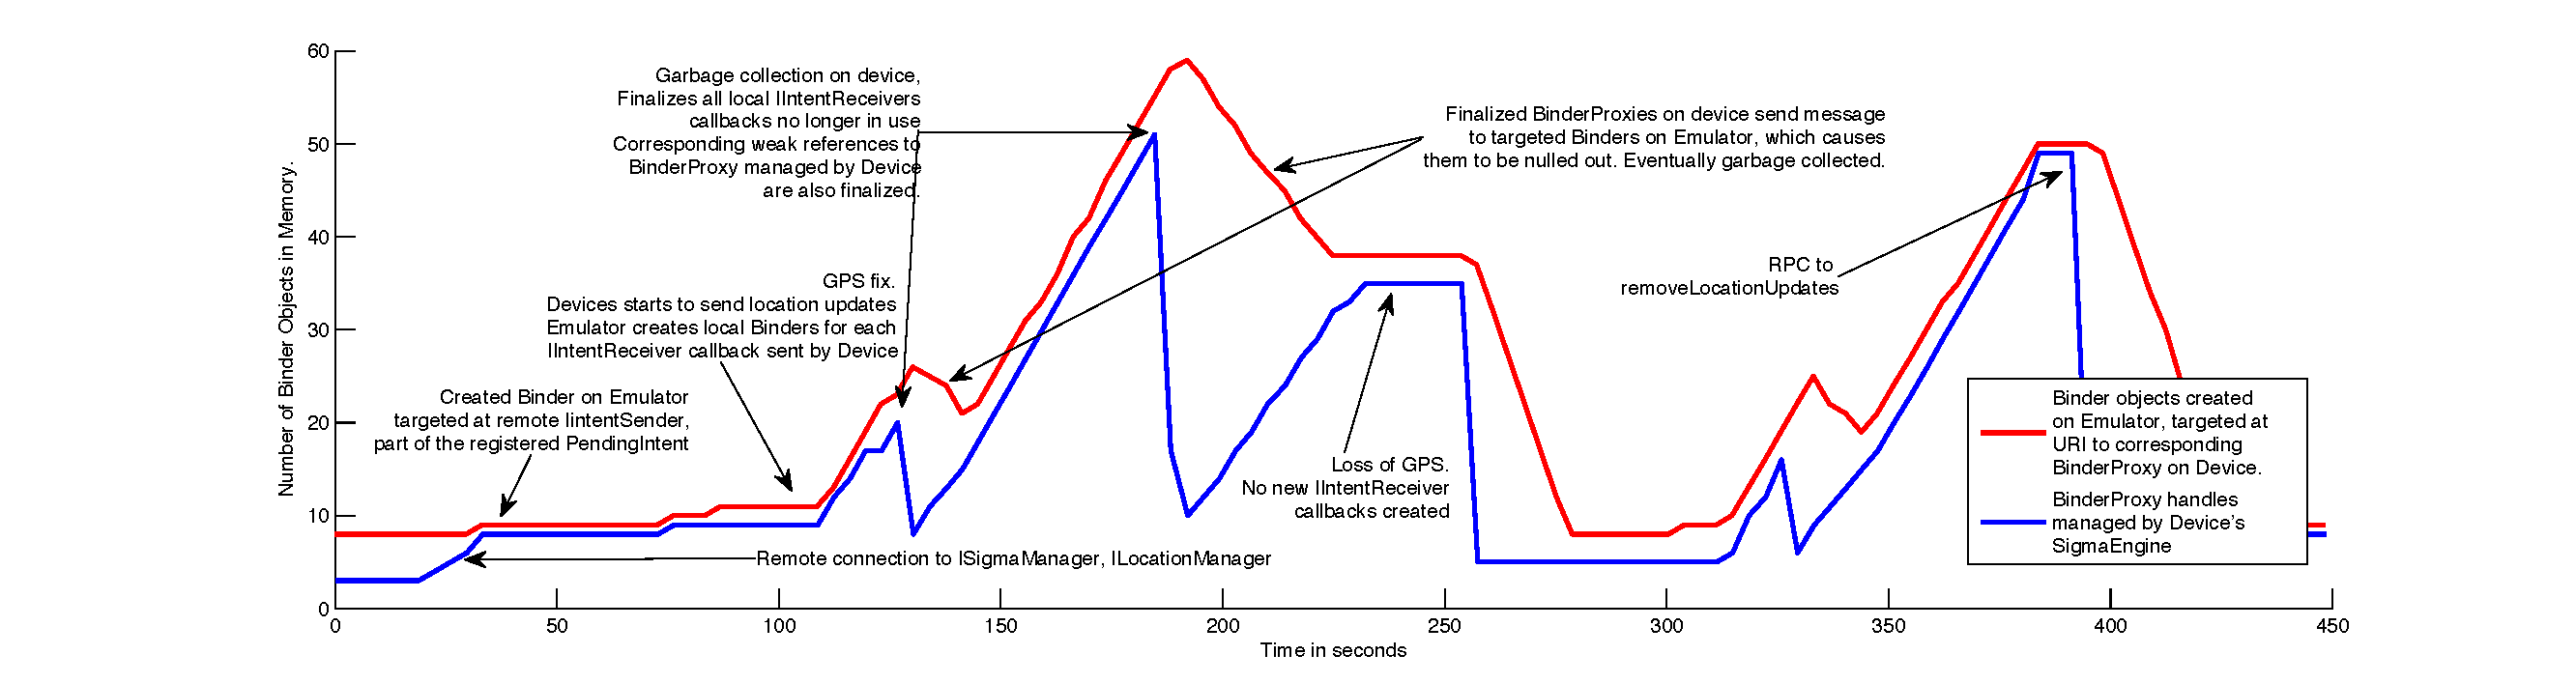
\includegraphics[width=\textwidth]{plots/location_sharing_reference_counting.pdf}
\caption{Management (reference counting) of Binder between Emulator and Nexus 4 device in the process of Emulator receiving location updates from Device via PendingIntent callbacks}
\label{fig:reference_counting}
\end{figure}

\subsubsection{Remote Sensor Events}
\label{sec:sensorevent}
The request to register for sensor events creates a SensorEventConnection which contains a BitTube object that is essentially an OO version of unix domain sockets. In establishing a SensorEventConnection, the file descriptor for the unix domain socket is communicated via binder. Subsequent communication happens through this socket, sent as atomic SensorEvent messages. This test demonstrates that socket messages are appropriately forwarded and received by Sigma. One performance measure is the difference between the time the native SensorEventListener callback receives a SensorEvent and the time remotely-routed SensorEventListener callback receives the corresponding SensorEvent message. Such timing is possible since each SensorEvent message has an identifying timestamp. Of course, the data channel used will have an impact on delay, and so we plot the results from using different data channels in figure~\ref{fig:sensorevent}.

From profiling, it turns out that the implementation of the HTTP server is to blame for the dramatic increase in latency going from a local binder-based data channel to one using the HTTP data channel. The local data channel uses an average of ~5\% CPU on a Nexus 4 device while sending sensor events, whereas the HTTP data channel uses an average of ~47\% CPU doing the same. The Sigma Engine itself uses the same ~10\% CPU regardless of choice of data channel. The NanoHTTPD~\cite{NanoHttpd} server we have chosen for the HTTP implementation is not very efficient. Each SensorEvent message causes a new POST request, and each request spawns a new thread. This behavior causes dozens of context switches each second, as SensorEvent messages are generated at ~10-30Hz, depending on parameters.

\begin{figure}[h]
\centering
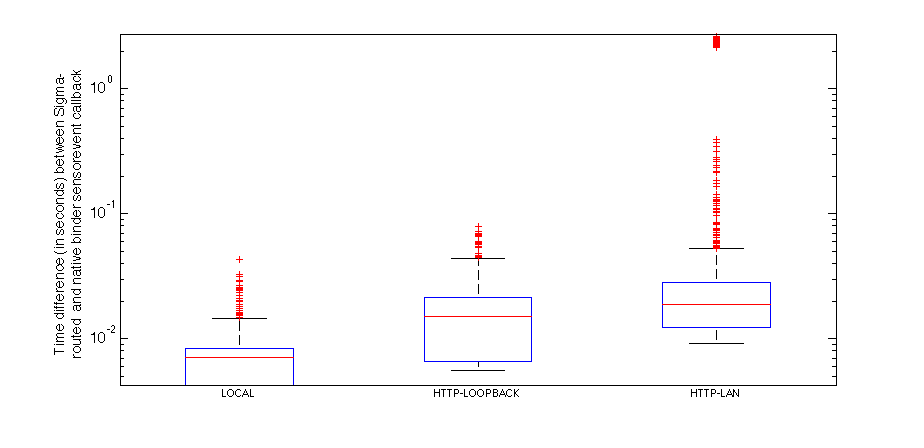
\includegraphics[width=0.7\textwidth]{plots/sensorevent_delay.png}
\caption{Distribution of delay in receiving SensorEvents remotely routed compared to locally routed, evaluation setup detailed in section~\ref{sec:sensorevent}}
\label{fig:sensorevent}
\end{figure}

Because there is also jitter in received sensor events, it is necessary to depend on the timestamp provided by the SensorEvent and not the timestamp of when the event is received by the listener callback. Also, depending on network conditions, it may not be possible to send sensor events at the full rate. Below we have simulated a limited bandwidth situation by routing HTTP packets through a rate limited proxy. Figure~\ref{fig:jitter} shows delay for each SensorEvent message as a function of timestamp. We see that as packets start to get queued at the proxy, the delay increases to a point where packets are dropped or never make it back to the device (discontinuities in the function).

\begin{figure}[h]
\centering
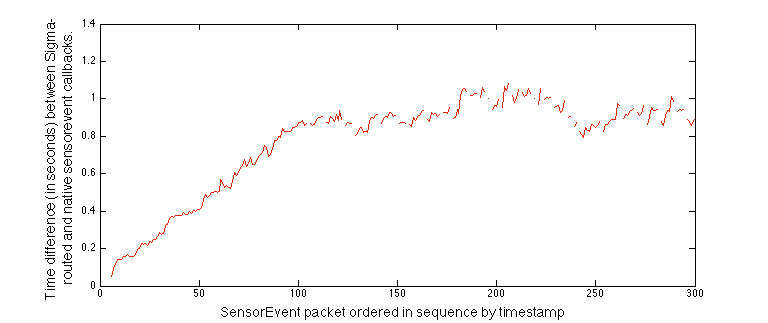
\includegraphics[width=0.7\textwidth]{plots/limited_bandwidth_increasing_latency.png}
\caption{Delay in receiving SensorEvents remotely routed through a rate-limited proxy, compared to locally routed. Plotted as a function of timestamp, discontinuities indicate that no remotely routed SensorEvent was received.}
\label{fig:jitter}
\end{figure}

These types of conditions are not typically expected in local Binder services, and it is a potential drawback to using Binder services for distributed communication as there is no inherent mechanism to detect nor manage such conditions. In any case, streaming frequent events of small packet sizes via Sigma may require a more streamlined implementation of the underlying data channel.

\section{Picture Sharing: A Distributed Application Purely in Android Binder}

\begin{snippet}
interface IPictureChatServer {
  // Returns a fileDescriptor to which caller writes picture data.
  // Server polls the fileDescriptor to locally receives picture.
  // Sigma takes care of proxying file descriptor over network.
  // Also returns (modifies) PictureEntry with metadata as a new id for picture
  // used for subsequent request to the server.
  ParcelFileDescriptor /* readFrom */ requestPicturePut(
    ISigmaManager caller, inout PictureEntry entry);

  // Client passes in fileDescriptor to which server will write picture data.
  PictureEntry requestPictureGet(
    ISigmaManager caller, String uuid, in ParcelFileDescriptor writeTo);
}

class PictureEntry implements Parcelable {
    String uuid, from;
    int numBytes;
}
\end{snippet}

The design involves a single Binder service that acts as a picture server, this service can run on each device. Clients connect to a remote picture server to upload (or share) a picture. The service interface could have been one that receives the picture as single large byte array. However, to make the implementation more interesting as a test, the PictureChatServer operates on put- and get- requests which operate on returned or passed-in file descriptors, respectively. Picture data is communicated from one end to the other by performing IO on these file descriptors

The PictureChatServer inherently (via native binder) allows different processes on the same device to bind with it, and put or get pictures. With Sigma an app on a remote device can access the same PictureChatServer service to put or get pictures. Thus, a picture sharing app can be implemented. Screenshots of an example application is provided in figure~\ref{fig:ExampleApplication}.

\begin{figure}[h]
\centering
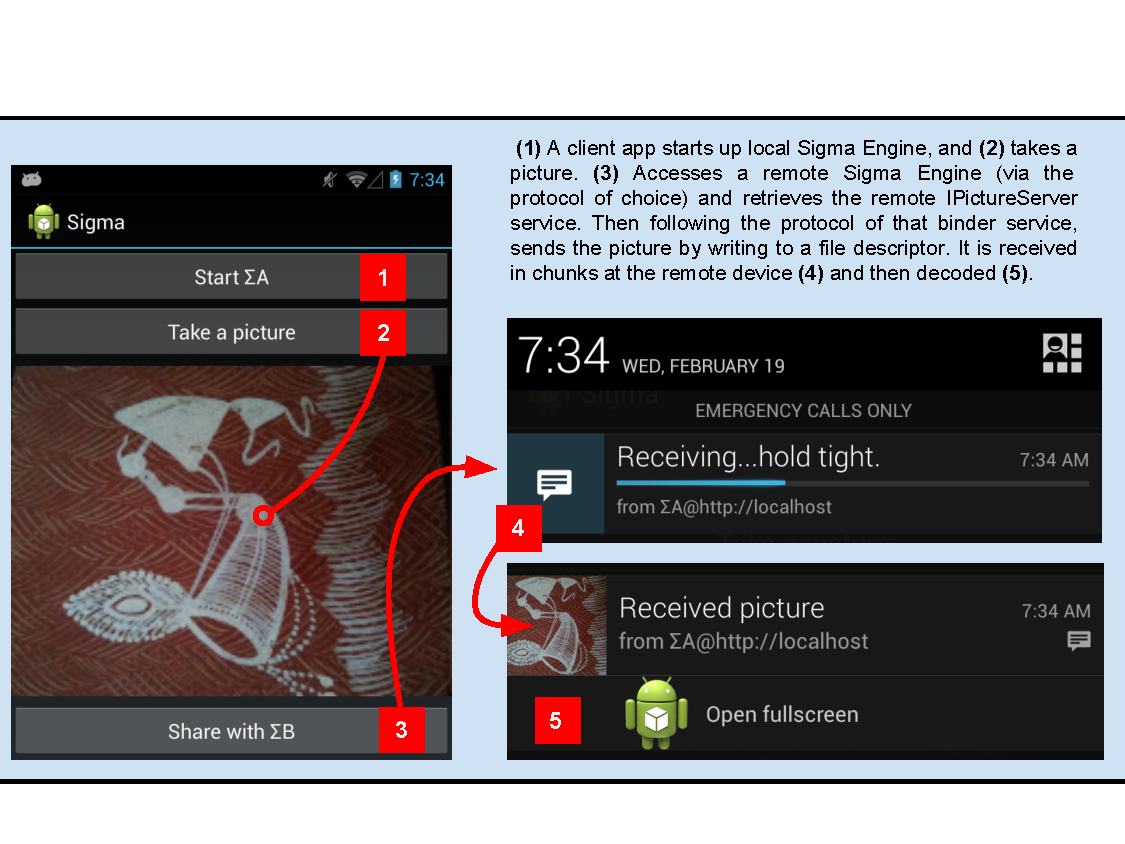
\includegraphics[width=\textwidth]{drawings/PictureChatExample.pdf}
\caption{Screenshots from simple picture sharing service}
\label{fig:ExampleApplication}
\end{figure}

Additionally, we can require that the caller Sigma Engine be passed in as an argument (i.e. the ``ISigmaManager caller'' argument). This way, the PictureChatServer can invoke RPCs on it to get details about the caller and his credentials. Right now, support is rudimentary, and we use it to get the name and protocol of the remote caller. In the future, we expect this mechanism is useful to authenticate and restrict callers.

\section{Discussion and next steps}
\label{sec:Discussion}
Sigma is not a finished product, nor is it the ultimate distributed communication mechanism. Rather it is a good starting point for experimentation with Binder as a distributed communication mechanism. There are still some deficiencies that need to be fixed up, and important features of Binder remain unimplemented.

\subsubsection{Sigma as it is implemented today is not compatible with standard Android}
We have implemented Sigma as an Android APK that can be installed on all devices. First issue: much of the internal Java Android Runtime is hidden in the SDK, but fortunately is accessible to applications by employing reflection. Many features of Sigma are implemented this way, but is unsupported and not a stable API. For instance, here's how we retrieve the internal ServiceManager from Java.

\begin{snippet}
IBinder binder = sigma.getServiceManager(remoteURI);
Object serviceManager = Class.forName("android.os.ServiceManagerNative")
                    .getMethod("asInterface", IBinder.class)
                    .invoke(null, binder);
\end{snippet}

The second and larger issue is: the OO Binder implementation encapsulates the internal structures that we need to access to correctly manage binder messages. For this we had to minimally modify the Android Runtime, and so Sigma is not compatible with the regular Android Runtime running on devices today--i.e. without resorting to extreme hacks (like poking into memory addresses~\cite{FacebookDalvikHacks}) to get at the same data. The necessary modifications are covered in Appendix~\ref{sec:AndroidRuntimeModifications}

\subsubsection{System services not portable across Android versions}
The RPC interface for the vast majority of system services is generated by the AIDL compiler--few like ServiceManager are hand-made. The generated RPC interfaces is not set in stone, it can vary with the different versions of the AIDL compiler or modifications to the AIDL source (like when switching the order of methods). For instance, a method foo() may be assigned code=1 in one version, and code=2 in another. Naturally, when operating between devices, identical RPC interfaces are expected by both ends. Generated AIDL interfaces do not have a notion of ``versions'' and it is impossible to tell from the Binder level whether two implementations of an interface (that go by the same name) have compatible internally generated structure. In testing, we have used the same version of Android among devices, compiled from the same source. So this issue was circumvented.

This limitation does not apply to RPC interfaces generated by third-party developers since they can fix a generated interface, ensuring backwards compatibility with previous versions by modifying the interface subsequently by hand.

\subsubsection{Parcels not portable between architectures}
Parcels were never implemented with the idea of portability. As we know, Parcels can contain binder objects and file descriptors which are obviously non-portable. Of course, the major implementation work in Sigma involved the managing of such objects, and provide a proxy for operating on them.

There is yet another aspect of Parcels that is non-portable, and this because primitive elements are represented in a long byte array, copied byte-for-byte. This operations happens preserves endianness, and this fact is troublesome since a remote device of the the opposite endianness would incorrectly process primitive data elements when it comes time to read each element out of the parcel. Although this is a seemingly major obstacle to the use of binder as a distributed communication mechanism, in practice we see that most all Android devices are ARM-based, and ARM chips are bi-endian (there is a little switch to toggle to specify the endianness). Android, by specification, is little-endian for all such ARM-based devices~\cite{ARMLittleEndian}.

There is a way to make parcels portable, but we leave that to future work. Parcels store offsets to objects contained within, but not offsets to other types of primitive data. We would first have to implement that feature (which will come with additional overhead in space requirements). To send over parcels, we would need to interpret each primitive element written into data array (is it an integer or a string of some length or something else?), marshalling each element in the Parcel separately using a canonical choice for endianness. Then on the other side, unmarshalling back into the data array would need to follow an analogous reverse procedure, decoding each element into the endianness appropriate for that system.

\subsubsection{XMPP and HTTP are not entirely satisfactory as data channels}
HTTP is only suitable over the local network since a HTTP server running on a device behind NAT is not accessible by others without additional configuration. XMPP uses a central chat server (accessible to all other devices) as a middleman. Having such a middleman incurs a performance penalty, and possible privacy concerns.

There are new technologies such as WebRTC~\cite{GoogleTalkLibrary} that seek to establish fully peer-to-peer connections. A signaling channel such as XMPP is used first to exchange descriptors between devices, and then a central server (typically hosted publicly by a third-party) is involved in establishing a direct peer-to-peer connection. All subsequent communication is done via this connection. This same technology is used by Google Talk, and is soon going to become a W3C standard. Implementing and evaluating binder over network using webrtc data channels is left for future work.

\subsubsection{What happens when a remote binder dies? Or if the network channel disconnects?}
Binder supports via ``linkToDeath()'' the registering of callback that is invoked when the process hosting a remote binder unexpectedly dies. This is fortunate because we can use the same mechanism to notify of clients of a Sigma-managed Proxy Binder when networks disconnects. A ``linkToDeath'' is not mandatory for clients to use. Another feature of Android Binder is that a DeadObjectException is thrown when a RPC is invoked against a dead remote binder object. However, these two feature are not currently implemented in the prototype.

A final feature supported by Java Binder is handling exceptions that happen remotely. For instance, during a binder transaction an exception can be thrown by the remote process. This exception is written into the reply Parcel instead of the expected reply. Back at the Proxy, reading an exception throws an RemoteException. Since this is mechanism implemented through Binder messages exclusively, Sigma automatically supports such exception handling.

\subsubsection{Sigma disregards Android permissions model}
\label{sec:DealingWithAndroidPermissions}
Each Android app belongs to a distinct Java package--this is the permissions namespace of the app. The PackageManager keeps track of the set of permissions that are requested by the package and also holds a map of the user-id assigned to each active package. Android activities and services within a package run as one or more processes which share the same user-id.

System services typically run as the root user. When an app (the caller) uses Binder IPC to make a call to another process like a system service, the callee can look up the process-id and user-id of the caller. This facility is baked into the BKM which is the component that handles the context switch from the caller to the callee (i.e. the caller thread sleeps, and wakes up a receiving thread in the callee's process). The callee can figure out (with the help of PackageManager) whether the caller has permission to access that particular system service. The system service in this way can reject unauthorized calls. This is a runtime security feature provided by BKM.

When the caller happens to be a process on a remote device, the Android security model breaks down. As implemented now, binder services are accessed and bound to the Sigma Engine, and not the process on the local device. The latter option does not make sense anyway since the remote ActivityManager does not know about the local process. Right now, Android permissions are effectively circumvented by having the Sigma Engine declaring all permissions--i.e. it essentially runs with root permissions. Any security is implemented separately by the Sigma Engine. And the permissions declared by the local process do not come into play.

There are obvious concerns with running with full permissions. One idea would be the remote device to communicate with the PackageManager on the local device, and grant an app all the permissions it is granted on the local device. However, this solution does not seem entirely satisfactory. Imagine an application requesting permission to access location of the local (its own) device means that it can also access location on all other remote devices.

It makes more sense for an app to be given permission to use a set of local services, and then a separate set of permissions granted to use remote services. For instance, a configuration panel on the remote device, much like a firewall, can be used to allow other devices access to certain services. Whenever the PackageManager is tasked with checking permissions for a binder object owned by Sigma Engine, such requests are redirected to Sigma. The implementation of such a panel and the necessary modifications to PackageManager is left for future work.

\subsection{Next Steps}
\label{sec:NextSteps}
In the long-term, it would be interesting to tightly couple two devices merging their Android Runtime state. Imagine that the local and remote PackageManager merge and present each device's components in their own namespace--one local, the other remote. Permissions to access services would have to be specified with the idea of a local and remote namespace as well. Consider also that the ActivityManager is merged. Sigma Engine would run within the runtime as part of the ActivityManager rather than as a separate package. With such tight coupling established, local components are able to connect to remote components directly through the ActivityManager's bindService(), the only difference is that apps specify a "remote" or "local" namespace to connect with. Tight coupling also solves some issues with notifications of binder service death. Life-cycle events of Android components on one device would automatically notify the other device, etc.

\pagebreak[4]
\section{Appendix}

\subsection{Necessary Modifications to the Android Runtime}
\label{sec:AndroidRuntimeModifications}
Binder services are often implemented in Java with AIDL-specified interfaces. But not always. Binder services can also be hand-made (in c, c++, or java) following any arbitrary convention for doing RPC. A binder service simply has to use the BKM in some way to qualify as one. Fortunately, all Android binder services follow the IBinder interface. So the goal of Sigma is to proxy all methods of the IBinder interface. Also fortunately, the Java and C++ versions of IBinder specify identical interfaces that are compatible with one another. In fact the Java implementation is really a JNI-based wrapper of the C++ version. Thus, native services can be made into Java BinderProxy objects by initializing them with a native service.

Unfortunately, the implementation of Java Binder and BinderProxy does not expose native handles to BBinder and BpBinder. In addition, there is no method to create Java Binder objects out of native handles. So if we are to implement Sigma in pure Java as it is, we have no hope of creating proxy interfaces to native binder services. An example of such a service is the SensorService. The remedy is to modify the Android Runtime. The following are signatures of added methods that do the job of converting from native binder to Java binder and vica-versa.

\begin{snippet}
class BinderInternal {
  // ...
  native IBinder binderForNativeHandle(int handle);
  native int nativeHandleForBinder(IBinder binder);
}
\end{snippet}

Binder transactions operate on binder\_io arguments which may contain objects and file descriptors. The BKM specially rewrites these objects, and so the binder\_io data structure has an offsets array containing information about where each object or file descriptor is in the data array. It follows that Sigma, in proxying binder transactions, also has to specially manage such arguments--these details we will leave for the next section. As a first requirement though, we need to access the offsets array from Java--where Sigma is implemented. Unfortunately, the Java and C++ Parcel objects which encapsulate the binder\_io data structure prevents access to this very important offsets array. Without it, we cannot know where and how may objects are in contained in the Parcel. Because this is an essential requirement, and we resort to modify or add methods to the Android Runtime to allow access.

\begin{snippet}
class Parcel {
  public static byte[] marshall();
  public static void unmarshall(byte[] data, int offset, int length);
  public static int[] getObjectPositions();
}
\end{snippet}

The marshall() and unmarshall() methods are already present in the default Parcel implementation, but it cannot handle Parcels that contain objects elements--we have fixed it to not care about that. The getObjectPositions() method is new it simply provides access to the underlying offsets array.

\begin{snippet}
parcel.setDataPosition(offset);
IBinder binder = parcel.readStrongBinder();
\end{snippet}

The source code to the modified Android Runtime is available online, see Appendix~\ref{app:SourceCode}. It is available as a patch for a particular version (4.2.2) of Android, but these changes should be compatible with the vast majority of Android versions with only minor modifications. The rest of the paper assumes a that we operate on the modified runtime.

\subsection{Links to source code, available online}
\label{app:SourceCode}

\subsubsection{Sigma Engine and example applications}
The main Sigma Engine that can be compiled into an Android package (or APK) can be found online. This includes all the examples from the Performance and Evaluation sections, including the Picture Sharing service.t

\noindent~The root Sigma project with dependencies: \verb|https://github.com/kastur/SigmaRoot|.

\noindent~Or, without the dependencies at: \verb|https://github.com/kastur/Sigma|.

\noindent~The XMPP library is patched slightly, and is online: \verb|https://github.com/kastur/ASmack|

The code has been tested on a modified Android Runtime with a Android base version 4.2.2\_r1 on the Android Emulator and Nexus 4 device.

\subsubsection{Modifications to the Android Runtime}
Of course, the Sigma Android package will not function on a regular Android device. We have modified the Android 4.2.2\_r1 version source tree to support some features. The modified runtime can be compiled and flashed on a real device or run on the emulator by following the directions at \verb|https://source.android.com/|. The following patches have to be applied to 2 modified sub-projects. The modified source tree for 2 sub-projects is available online:

\begin{Verbatim}
https://github.com/6b72/platform_frameworks_base/tree/sigma
https://github.com/6b72/platform_frameworks_native/tree/sigma
\end{Verbatim}

\noindent~The same modifications can be viewed as a patch to the baseline 4.2.2\_r1 version.
\begin{Verbatim}
https://github.com/6b72/platform_frameworks_base/compare/
763ef60466ac752a3031719fb86b08486c9946b1...3ae311d29691b3060e67bae1c891fb8fbbc1be0f

https://github.com/6b72/platform_frameworks_native/compare/
529cb9ed9c5d62d5b270cdd650380ae116382143...994ae7fa16165b3e85553d154111df0a2f5a5af3
\end{Verbatim}

\pagebreak[4]
\subsection{The Binder Kernel Module's binder\_call and handler function}
\label{app:binder_call}

\begin{snippet}
binder_call(binder_state *bs, binder_io *msg, binder_io *reply, void *target, int code)

bs -     each binder transaction and service gets its own state.
         Essentially contains a file descriptor to the binder kernel module.

msg -    essentially contains a data array with the following:
         * "android.os.IServiceManager" - name of the interface published in
                                          target binder service.
          * "com.example.service"       - name of the service to be  published
          * binder_service              - reference to the local binder
                                          service

reply -   contains the returned data array after the transaction. Can be null
          if there is no return value or we don't care about it.

target -  is a reference to a remote binder service already published. Usually
          references are obtained by a binder_call to the ServiceManager to retrieve
          published services. However, we can always make a binder call to the
          ServiceManager itself, which is always at the address (void*)0.

code -    is a non-specific value passed to the handler of the remote binder object.
          In this case, we pass an integer representing the action to be performed,
          where SVC_MGR_ADD_SERVICE is an predefined int.
\end{snippet}

All operations of a binder\_service are implemented inside of a handler function; the function signature resembles that of binder\_call:

\begin{snippet}
service_handler(binder_state *bs, binder_txn *txn,  binder_io *msg, binder_io *reply)
bs -      The initiating transaction.
txn -     essentially contains code (from binder_call), and the calling uid and pid.
msg -     The incoming message from binder_call.
reply -   The return value should be written out here, if any
\end{snippet}

\subsection{The binder\_io struct}
\label{app:binder_io}
The binder\_io struct holds the data for binder transactions as byte arrays, and it used by the BKM. Binder objects and file descriptors are flattened as flat\_binder\_object data structures and written into the data array, with the offset for each object written stored in the offs array. Remote binder objects are local descriptors that refer to records managed within the BKM.

The Java and C++ binder transactions operate on Parcel objects which encapsulate a binder\_io data structure.

\begin{snippet}
struct binder_io {
  char *data;            /* start of data buffer */
  uint32_t *offs;        /* array of offsets */
  uint32_t data_avail;   /* bytes available in data buffer */
  uint32_t offs_avail;   /* entries available in offsets array */
};
\end{snippet}

This struct holds either a local pointer to a binder service or a kernel-module provided handle. This same struct is used for storing file descriptors as well.

\begin{snippet}
struct flat_binder_object {
  unsigned long type, flags  /* header */
  union {
    void *binder;        /* local object */
    signed long handle;  /* remote object */
  };
  void *cookie;          /* extra data */
};
\end{snippet}

\subsection{IServiceManager's object-oriented service interface}
\label{app:ServiceManager}

\begin{snippet}
class IServiceManager : public IInterface {
 public:
    // Retrieve an existing service, blocking for a few seconds if it doesn't yet exist.
  virtual sp<IBinder> getService(const String16& name) const = 0;
    // Retrieve an existing service, non-blocking.
  virtual sp<IBinder> checkService(const String16& name) const = 0;
    // Register a service.
  virtual status_t addService(const String16& name, const sp<IBinder>& service, ..) = 0;
    // Return list of all existing services.
  virtual Vector<String16> listServices() = 0;
}
\end{snippet}

Note that what is not captured by the interface definition alone is that arbitrary process do not have permission to add new services. Inside the invocation of addService is a call to getCallingUid(), which is used to enforce permissions, limiting it so that only system processes may add services.

getCallingUid() and getCallingPid() are features of the Binder Kernel Module to get information about the caller process.

\pagebreak[4]
\subsection{Examples of Sigma (Wire) messages}
\label{app:WireExchange}
The following set of figures show in detail the Wire messages exchanged between two Sigma Engines (implemented via a LOCAL protocol, with engines running on same device and communicating to each other via native binder). The messages correspond to the example from the beginning of "Design of Sigma" section, where a remote Sigma Engine reference is first retrieved via RPC to a local Sigma Engine, and then a reference to remote service is obtained.

\begin{figure}[h!]
\centering
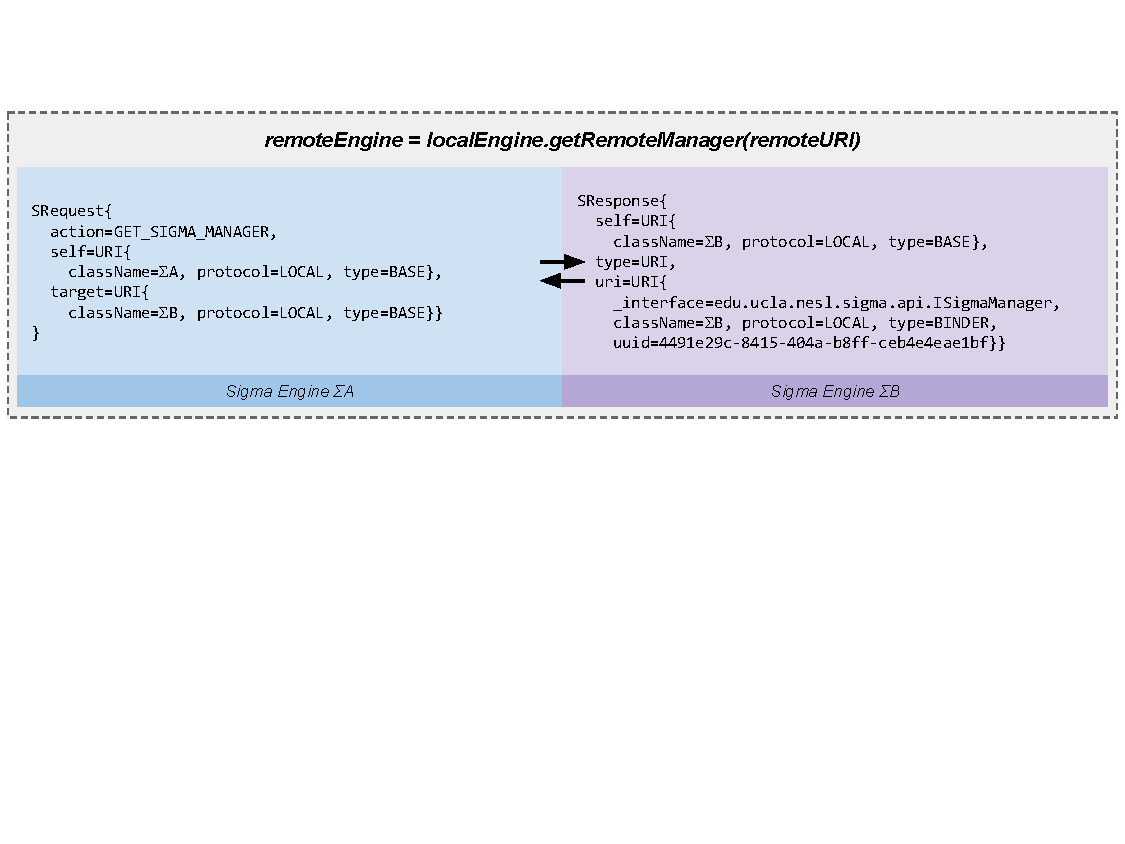
\includegraphics[width=\textwidth]{drawings/WireExchange1.pdf}
\end{figure}

\begin{figure}[h!]
\centering
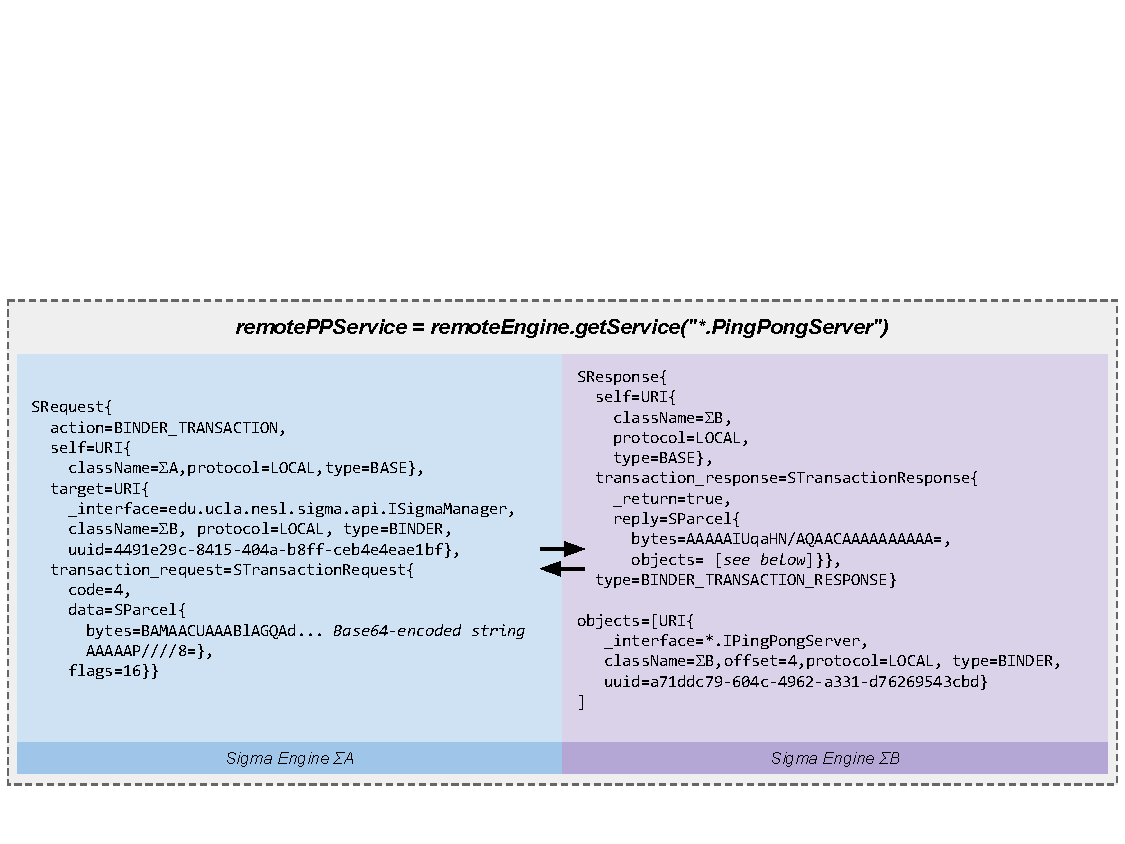
\includegraphics[width=\textwidth]{drawings/WireExchange2.pdf}
\end{figure}

Here, since we are operating under the LOCAL protocol, all transactions proxy binder objects are transit through the local Sigma Engine and then to the remote Sigma Engine (which also runs on the same device as a different process), and then from there to the native binder service. Naturally this the transit from local to remote Sigma Engine will take over the network (through HTTP or XMPP) for those implementations.

\pagebreak[4]
\subsection{Wire messages exchanged during a recursive binder RPC}
\label{app:WireExchangeRecursive}
An exchange of Wire messages detailing a recursive binder that take place between two Sigma Engine instances from the example of the PingPong service.
\begin{figure}[h!]
\centering
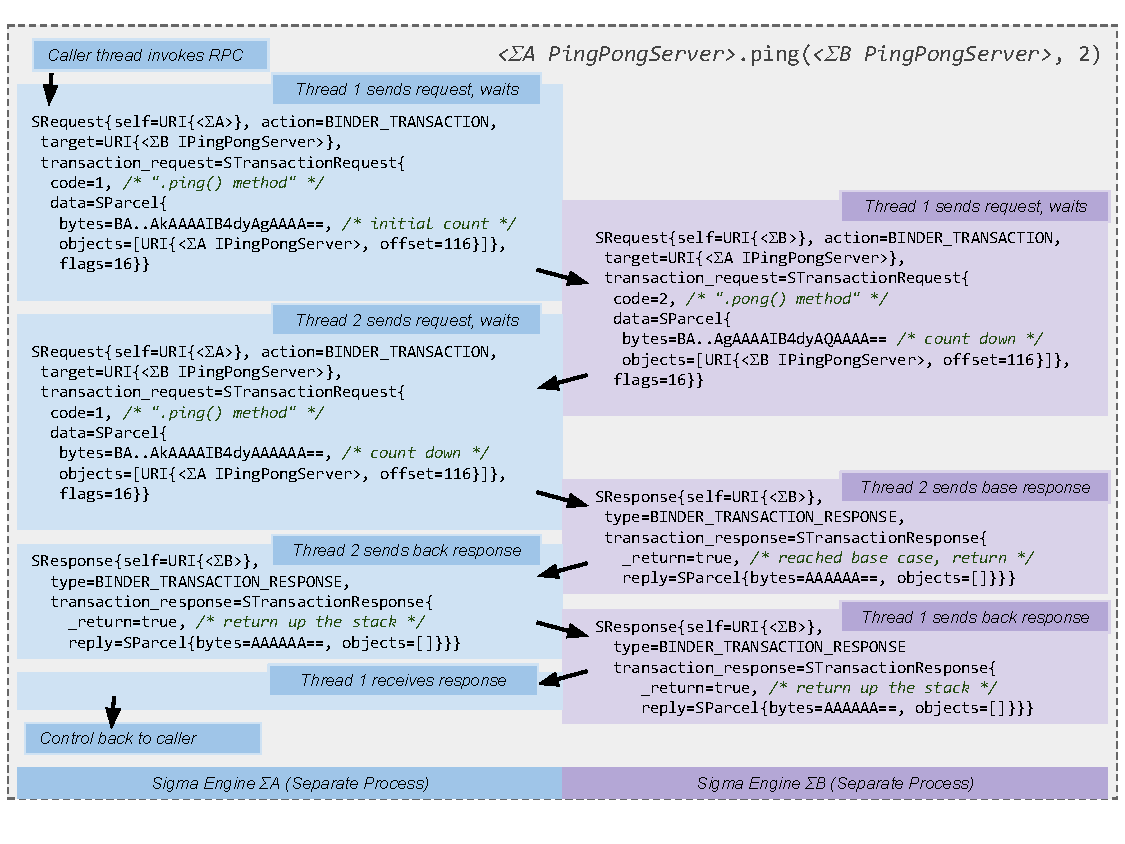
\includegraphics[width=\textwidth]{drawings/WireExchangeRecursive.pdf}
\end{figure}
\pagebreak[4]

\bibliography{sigma}

\end{document}
